\documentclass{report}

%%%%%%%%%%%%%%%%%%%%%%%%%%%%%%%%%
% PACKAGE IMPORTS
%%%%%%%%%%%%%%%%%%%%%%%%%%%%%%%%%


\usepackage[tmargin=2cm,rmargin=1in,lmargin=1in,margin=0.85in,bmargin=2cm,footskip=.2in]{geometry}
\usepackage{amsmath,amsfonts,amsthm,amssymb,mathtools}
\usepackage[varbb]{newpxmath}
\usepackage{xfrac}
\usepackage[makeroom]{cancel}
\usepackage{mathtools}
\usepackage{bookmark}
\usepackage{enumitem}
\usepackage{hyperref,theoremref}
\hypersetup{
	pdftitle={Assignment},
	colorlinks=true, linkcolor=doc!90,
	bookmarksnumbered=true,
	bookmarksopen=true
}
\usepackage[most,many,breakable]{tcolorbox}
\usepackage{xcolor}
\usepackage{varwidth}
\usepackage{varwidth}
\usepackage{etoolbox}
%\usepackage{authblk}
\usepackage{nameref}
\usepackage{multicol,array}
\usepackage{tikz-cd}
\usepackage[ruled,vlined,linesnumbered]{algorithm2e}
\usepackage{comment} % enables the use of multi-line comments (\ifx \fi) 
\usepackage{import}
\usepackage{xifthen}
\usepackage{pdfpages}
\usepackage{transparent}

\newcommand\mycommfont[1]{\footnotesize\ttfamily\textcolor{blue}{#1}}
\SetCommentSty{mycommfont}
\newcommand{\incfig}[1]{%
    \def\svgwidth{\columnwidth}
    \import{./figures/}{#1.pdf_tex}
}

\usepackage{tikzsymbols}
\renewcommand\qedsymbol{$\Laughey$}


%\usepackage{import}
%\usepackage{xifthen}
%\usepackage{pdfpages}
%\usepackage{transparent}


%%%%%%%%%%%%%%%%%%%%%%%%%%%%%%
% SELF MADE COLORS
%%%%%%%%%%%%%%%%%%%%%%%%%%%%%%



\definecolor{myg}{RGB}{56, 140, 70}
\definecolor{myb}{RGB}{45, 111, 177}
\definecolor{myr}{RGB}{199, 68, 64}
\definecolor{mytheorembg}{HTML}{F2F2F9}
\definecolor{mytheoremfr}{HTML}{00007B}
\definecolor{mylenmabg}{HTML}{FFFAF8}
\definecolor{mylenmafr}{HTML}{983b0f}
\definecolor{mypropbg}{HTML}{f2fbfc}
\definecolor{mypropfr}{HTML}{191971}
\definecolor{myexamplebg}{HTML}{F2FBF8}
\definecolor{myexamplefr}{HTML}{88D6D1}
\definecolor{myexampleti}{HTML}{2A7F7F}
\definecolor{mydefinitbg}{HTML}{E5E5FF}
\definecolor{mydefinitfr}{HTML}{3F3FA3}
\definecolor{notesgreen}{RGB}{0,162,0}
\definecolor{myp}{RGB}{197, 92, 212}
\definecolor{mygr}{HTML}{2C3338}
\definecolor{myred}{RGB}{127,0,0}
\definecolor{myyellow}{RGB}{169,121,69}
\definecolor{myexercisebg}{HTML}{F2FBF8}
\definecolor{myexercisefg}{HTML}{88D6D1}


%%%%%%%%%%%%%%%%%%%%%%%%%%%%
% TCOLORBOX SETUPS
%%%%%%%%%%%%%%%%%%%%%%%%%%%%

\setlength{\parindent}{1cm}
%================================
% THEOREM BOX
%================================

\tcbuselibrary{theorems,skins,hooks}
\newtcbtheorem[number within=section]{Theorem}{Theorem}
{%
	enhanced,
	breakable,
	colback = mytheorembg,
	frame hidden,
	boxrule = 0sp,
	borderline west = {2pt}{0pt}{mytheoremfr},
	sharp corners,
	detach title,
	before upper = \tcbtitle\par\smallskip,
	coltitle = mytheoremfr,
	fonttitle = \bfseries\sffamily,
	description font = \mdseries,
	separator sign none,
	segmentation style={solid, mytheoremfr},
}
{th}

\tcbuselibrary{theorems,skins,hooks}
\newtcbtheorem[number within=chapter]{theorem}{Theorem}
{%
	enhanced,
	breakable,
	colback = mytheorembg,
	frame hidden,
	boxrule = 0sp,
	borderline west = {2pt}{0pt}{mytheoremfr},
	sharp corners,
	detach title,
	before upper = \tcbtitle\par\smallskip,
	coltitle = mytheoremfr,
	fonttitle = \bfseries\sffamily,
	description font = \mdseries,
	separator sign none,
	segmentation style={solid, mytheoremfr},
}
{th}


\tcbuselibrary{theorems,skins,hooks}
\newtcolorbox{Theoremcon}
{%
	enhanced
	,breakable
	,colback = mytheorembg
	,frame hidden
	,boxrule = 0sp
	,borderline west = {2pt}{0pt}{mytheoremfr}
	,sharp corners
	,description font = \mdseries
	,separator sign none
}

%================================
% Corollery
%================================
\tcbuselibrary{theorems,skins,hooks}
\newtcbtheorem[number within=section]{Corollary}{Corollary}
{%
	enhanced
	,breakable
	,colback = myp!10
	,frame hidden
	,boxrule = 0sp
	,borderline west = {2pt}{0pt}{myp!85!black}
	,sharp corners
	,detach title
	,before upper = \tcbtitle\par\smallskip
	,coltitle = myp!85!black
	,fonttitle = \bfseries\sffamily
	,description font = \mdseries
	,separator sign none
	,segmentation style={solid, myp!85!black}
}
{th}
\tcbuselibrary{theorems,skins,hooks}
\newtcbtheorem[number within=chapter]{corollary}{Corollary}
{%
	enhanced
	,breakable
	,colback = myp!10
	,frame hidden
	,boxrule = 0sp
	,borderline west = {2pt}{0pt}{myp!85!black}
	,sharp corners
	,detach title
	,before upper = \tcbtitle\par\smallskip
	,coltitle = myp!85!black
	,fonttitle = \bfseries\sffamily
	,description font = \mdseries
	,separator sign none
	,segmentation style={solid, myp!85!black}
}
{th}


%================================
% LENMA
%================================

\tcbuselibrary{theorems,skins,hooks}
\newtcbtheorem[number within=section]{Lenma}{Lenma}
{%
	enhanced,
	breakable,
	colback = mylenmabg,
	frame hidden,
	boxrule = 0sp,
	borderline west = {2pt}{0pt}{mylenmafr},
	sharp corners,
	detach title,
	before upper = \tcbtitle\par\smallskip,
	coltitle = mylenmafr,
	fonttitle = \bfseries\sffamily,
	description font = \mdseries,
	separator sign none,
	segmentation style={solid, mylenmafr},
}
{th}

\tcbuselibrary{theorems,skins,hooks}
\newtcbtheorem[number within=chapter]{lenma}{Lenma}
{%
	enhanced,
	breakable,
	colback = mylenmabg,
	frame hidden,
	boxrule = 0sp,
	borderline west = {2pt}{0pt}{mylenmafr},
	sharp corners,
	detach title,
	before upper = \tcbtitle\par\smallskip,
	coltitle = mylenmafr,
	fonttitle = \bfseries\sffamily,
	description font = \mdseries,
	separator sign none,
	segmentation style={solid, mylenmafr},
}
{th}


%================================
% PROPOSITION
%================================

\tcbuselibrary{theorems,skins,hooks}
\newtcbtheorem[number within=section]{Prop}{Proposition}
{%
	enhanced,
	breakable,
	colback = mypropbg,
	frame hidden,
	boxrule = 0sp,
	borderline west = {2pt}{0pt}{mypropfr},
	sharp corners,
	detach title,
	before upper = \tcbtitle\par\smallskip,
	coltitle = mypropfr,
	fonttitle = \bfseries\sffamily,
	description font = \mdseries,
	separator sign none,
	segmentation style={solid, mypropfr},
}
{th}

\tcbuselibrary{theorems,skins,hooks}
\newtcbtheorem[number within=chapter]{prop}{Proposition}
{%
	enhanced,
	breakable,
	colback = mypropbg,
	frame hidden,
	boxrule = 0sp,
	borderline west = {2pt}{0pt}{mypropfr},
	sharp corners,
	detach title,
	before upper = \tcbtitle\par\smallskip,
	coltitle = mypropfr,
	fonttitle = \bfseries\sffamily,
	description font = \mdseries,
	separator sign none,
	segmentation style={solid, mypropfr},
}
{th}


%================================
% CLAIM
%================================

\tcbuselibrary{theorems,skins,hooks}
\newtcbtheorem[number within=section]{claim}{Claim}
{%
	enhanced
	,breakable
	,colback = myg!10
	,frame hidden
	,boxrule = 0sp
	,borderline west = {2pt}{0pt}{myg}
	,sharp corners
	,detach title
	,before upper = \tcbtitle\par\smallskip
	,coltitle = myg!85!black
	,fonttitle = \bfseries\sffamily
	,description font = \mdseries
	,separator sign none
	,segmentation style={solid, myg!85!black}
}
{th}



%================================
% Exercise
%================================

\tcbuselibrary{theorems,skins,hooks}
\newtcbtheorem[number within=section]{Exercise}{Exercise}
{%
	enhanced,
	breakable,
	colback = myexercisebg,
	frame hidden,
	boxrule = 0sp,
	borderline west = {2pt}{0pt}{myexercisefg},
	sharp corners,
	detach title,
	before upper = \tcbtitle\par\smallskip,
	coltitle = myexercisefg,
	fonttitle = \bfseries\sffamily,
	description font = \mdseries,
	separator sign none,
	segmentation style={solid, myexercisefg},
}
{th}

\tcbuselibrary{theorems,skins,hooks}
\newtcbtheorem[number within=chapter]{exercise}{Exercise}
{%
	enhanced,
	breakable,
	colback = myexercisebg,
	frame hidden,
	boxrule = 0sp,
	borderline west = {2pt}{0pt}{myexercisefg},
	sharp corners,
	detach title,
	before upper = \tcbtitle\par\smallskip,
	coltitle = myexercisefg,
	fonttitle = \bfseries\sffamily,
	description font = \mdseries,
	separator sign none,
	segmentation style={solid, myexercisefg},
}
{th}

%================================
% EXAMPLE BOX
%================================

\newtcbtheorem[number within=section]{Example}{Example}
{%
	colback = myexamplebg
	,breakable
	,colframe = myexamplefr
	,coltitle = myexampleti
	,boxrule = 1pt
	,sharp corners
	,detach title
	,before upper=\tcbtitle\par\smallskip
	,fonttitle = \bfseries
	,description font = \mdseries
	,separator sign none
	,description delimiters parenthesis
}
{ex}

\newtcbtheorem[number within=chapter]{example}{Example}
{%
	colback = myexamplebg
	,breakable
	,colframe = myexamplefr
	,coltitle = myexampleti
	,boxrule = 1pt
	,sharp corners
	,detach title
	,before upper=\tcbtitle\par\smallskip
	,fonttitle = \bfseries
	,description font = \mdseries
	,separator sign none
	,description delimiters parenthesis
}
{ex}

%================================
% DEFINITION BOX
%================================

\newtcbtheorem[number within=section]{Definition}{Definition}{enhanced,
	before skip=2mm,after skip=2mm, colback=red!5,colframe=red!80!black,boxrule=0.5mm,
	attach boxed title to top left={xshift=1cm,yshift*=1mm-\tcboxedtitleheight}, varwidth boxed title*=-3cm,
	boxed title style={frame code={
					\path[fill=tcbcolback]
					([yshift=-1mm,xshift=-1mm]frame.north west)
					arc[start angle=0,end angle=180,radius=1mm]
					([yshift=-1mm,xshift=1mm]frame.north east)
					arc[start angle=180,end angle=0,radius=1mm];
					\path[left color=tcbcolback!60!black,right color=tcbcolback!60!black,
						middle color=tcbcolback!80!black]
					([xshift=-2mm]frame.north west) -- ([xshift=2mm]frame.north east)
					[rounded corners=1mm]-- ([xshift=1mm,yshift=-1mm]frame.north east)
					-- (frame.south east) -- (frame.south west)
					-- ([xshift=-1mm,yshift=-1mm]frame.north west)
					[sharp corners]-- cycle;
				},interior engine=empty,
		},
	fonttitle=\bfseries,
	title={#2},#1}{def}
\newtcbtheorem[number within=chapter]{definition}{Definition}{enhanced,
	before skip=2mm,after skip=2mm, colback=red!5,colframe=red!80!black,boxrule=0.5mm,
	attach boxed title to top left={xshift=1cm,yshift*=1mm-\tcboxedtitleheight}, varwidth boxed title*=-3cm,
	boxed title style={frame code={
					\path[fill=tcbcolback]
					([yshift=-1mm,xshift=-1mm]frame.north west)
					arc[start angle=0,end angle=180,radius=1mm]
					([yshift=-1mm,xshift=1mm]frame.north east)
					arc[start angle=180,end angle=0,radius=1mm];
					\path[left color=tcbcolback!60!black,right color=tcbcolback!60!black,
						middle color=tcbcolback!80!black]
					([xshift=-2mm]frame.north west) -- ([xshift=2mm]frame.north east)
					[rounded corners=1mm]-- ([xshift=1mm,yshift=-1mm]frame.north east)
					-- (frame.south east) -- (frame.south west)
					-- ([xshift=-1mm,yshift=-1mm]frame.north west)
					[sharp corners]-- cycle;
				},interior engine=empty,
		},
	fonttitle=\bfseries,
	title={#2},#1}{def}



%================================
% Solution BOX
%================================

\makeatletter
\newtcbtheorem{question}{Question}{enhanced,
	breakable,
	colback=white,
	colframe=myb!80!black,
	attach boxed title to top left={yshift*=-\tcboxedtitleheight},
	fonttitle=\bfseries,
	title={#2},
	boxed title size=title,
	boxed title style={%
			sharp corners,
			rounded corners=northwest,
			colback=tcbcolframe,
			boxrule=0pt,
		},
	underlay boxed title={%
			\path[fill=tcbcolframe] (title.south west)--(title.south east)
			to[out=0, in=180] ([xshift=5mm]title.east)--
			(title.center-|frame.east)
			[rounded corners=\kvtcb@arc] |-
			(frame.north) -| cycle;
		},
	#1
}{def}
\makeatother

%================================
% SOLUTION BOX
%================================

\makeatletter
\newtcolorbox{solution}{enhanced,
	breakable,
	colback=white,
	colframe=myg!80!black,
	attach boxed title to top left={yshift*=-\tcboxedtitleheight},
	title=Solution,
	boxed title size=title,
	boxed title style={%
			sharp corners,
			rounded corners=northwest,
			colback=tcbcolframe,
			boxrule=0pt,
		},
	underlay boxed title={%
			\path[fill=tcbcolframe] (title.south west)--(title.south east)
			to[out=0, in=180] ([xshift=5mm]title.east)--
			(title.center-|frame.east)
			[rounded corners=\kvtcb@arc] |-
			(frame.north) -| cycle;
		},
}
\makeatother

%================================
% Question BOX
%================================

\makeatletter
\newtcbtheorem{qstion}{Question}{enhanced,
	breakable,
	colback=white,
	colframe=mygr,
	attach boxed title to top left={yshift*=-\tcboxedtitleheight},
	fonttitle=\bfseries,
	title={#2},
	boxed title size=title,
	boxed title style={%
			sharp corners,
			rounded corners=northwest,
			colback=tcbcolframe,
			boxrule=0pt,
		},
	underlay boxed title={%
			\path[fill=tcbcolframe] (title.south west)--(title.south east)
			to[out=0, in=180] ([xshift=5mm]title.east)--
			(title.center-|frame.east)
			[rounded corners=\kvtcb@arc] |-
			(frame.north) -| cycle;
		},
	#1
}{def}
\makeatother

\newtcbtheorem[number within=chapter]{wconc}{Wrong Concept}{
	breakable,
	enhanced,
	colback=white,
	colframe=myr,
	arc=0pt,
	outer arc=0pt,
	fonttitle=\bfseries\sffamily\large,
	colbacktitle=myr,
	attach boxed title to top left={},
	boxed title style={
			enhanced,
			skin=enhancedfirst jigsaw,
			arc=3pt,
			bottom=0pt,
			interior style={fill=myr}
		},
	#1
}{def}



%================================
% NOTE BOX
%================================

\usetikzlibrary{arrows,calc,shadows.blur}
\tcbuselibrary{skins}
\newtcolorbox{note}[1][]{%
	enhanced jigsaw,
	colback=gray!20!white,%
	colframe=gray!80!black,
	size=small,
	boxrule=1pt,
	title=\textbf{Note:-},
	halign title=flush center,
	coltitle=black,
	breakable,
	drop shadow=black!50!white,
	attach boxed title to top left={xshift=1cm,yshift=-\tcboxedtitleheight/2,yshifttext=-\tcboxedtitleheight/2},
	minipage boxed title=1.5cm,
	boxed title style={%
			colback=white,
			size=fbox,
			boxrule=1pt,
			boxsep=2pt,
			underlay={%
					\coordinate (dotA) at ($(interior.west) + (-0.5pt,0)$);
					\coordinate (dotB) at ($(interior.east) + (0.5pt,0)$);
					\begin{scope}
						\clip (interior.north west) rectangle ([xshift=3ex]interior.east);
						\filldraw [white, blur shadow={shadow opacity=60, shadow yshift=-.75ex}, rounded corners=2pt] (interior.north west) rectangle (interior.south east);
					\end{scope}
					\begin{scope}[gray!80!black]
						\fill (dotA) circle (2pt);
						\fill (dotB) circle (2pt);
					\end{scope}
				},
		},
	#1,
}

%%%%%%%%%%%%%%%%%%%%%%%%%%%%%%
% SELF MADE COMMANDS
%%%%%%%%%%%%%%%%%%%%%%%%%%%%%%


\newcommand{\thm}[2]{\begin{Theorem}{#1}{}#2\end{Theorem}}
\newcommand{\cor}[2]{\begin{Corollary}{#1}{}#2\end{Corollary}}
\newcommand{\mlenma}[2]{\begin{Lenma}{#1}{}#2\end{Lenma}}
\newcommand{\mprop}[2]{\begin{Prop}{#1}{}#2\end{Prop}}
\newcommand{\clm}[3]{\begin{claim}{#1}{#2}#3\end{claim}}
\newcommand{\wc}[2]{\begin{wconc}{#1}{}\setlength{\parindent}{1cm}#2\end{wconc}}
\newcommand{\thmcon}[1]{\begin{Theoremcon}{#1}\end{Theoremcon}}
\newcommand{\ex}[2]{\begin{Example}{#1}{}#2\end{Example}}
\newcommand{\dfn}[2]{\begin{Definition}[colbacktitle=red!75!black]{#1}{}#2\end{Definition}}
\newcommand{\dfnc}[2]{\begin{definition}[colbacktitle=red!75!black]{#1}{}#2\end{definition}}
\newcommand{\qs}[2]{\begin{question}{#1}{}#2\end{question}}
\newcommand{\pf}[2]{\begin{myproof}[#1]#2\end{myproof}}
\newcommand{\nt}[1]{\begin{note}#1\end{note}}

\newcommand*\circled[1]{\tikz[baseline=(char.base)]{
		\node[shape=circle,draw,inner sep=1pt] (char) {#1};}}
\newcommand\getcurrentref[1]{%
	\ifnumequal{\value{#1}}{0}
	{??}
	{\the\value{#1}}%
}
\newcommand{\getCurrentSectionNumber}{\getcurrentref{section}}
\newenvironment{myproof}[1][\proofname]{%
	\proof[\bfseries #1: ]%
}{\endproof}

\newcommand{\mclm}[2]{\begin{myclaim}[#1]#2\end{myclaim}}
\newenvironment{myclaim}[1][\claimname]{\proof[\bfseries #1: ]}{}

\newcounter{mylabelcounter}

\makeatletter
\newcommand{\setword}[2]{%
	\phantomsection
	#1\def\@currentlabel{\unexpanded{#1}}\label{#2}%
}
\makeatother




\tikzset{
	symbol/.style={
			draw=none,
			every to/.append style={
					edge node={node [sloped, allow upside down, auto=false]{$#1$}}}
		}
}


% deliminators
\DeclarePairedDelimiter{\abs}{\lvert}{\rvert}
\DeclarePairedDelimiter{\norm}{\lVert}{\rVert}

\DeclarePairedDelimiter{\ceil}{\lceil}{\rceil}
\DeclarePairedDelimiter{\floor}{\lfloor}{\rfloor}
\DeclarePairedDelimiter{\round}{\lfloor}{\rceil}

\newsavebox\diffdbox
\newcommand{\slantedromand}{{\mathpalette\makesl{d}}}
\newcommand{\makesl}[2]{%
\begingroup
\sbox{\diffdbox}{$\mathsurround=0pt#1\mathrm{#2}$}%
\pdfsave
\pdfsetmatrix{1 0 0.2 1}%
\rlap{\usebox{\diffdbox}}%
\pdfrestore
\hskip\wd\diffdbox
\endgroup
}
\newcommand{\dd}[1][]{\ensuremath{\mathop{}\!\ifstrempty{#1}{%
\slantedromand\@ifnextchar^{\hspace{0.2ex}}{\hspace{0.1ex}}}%
{\slantedromand\hspace{0.2ex}^{#1}}}}
\ProvideDocumentCommand\dv{o m g}{%
  \ensuremath{%
    \IfValueTF{#3}{%
      \IfNoValueTF{#1}{%
        \frac{\dd #2}{\dd #3}%
      }{%
        \frac{\dd^{#1} #2}{\dd #3^{#1}}%
      }%
    }{%
      \IfNoValueTF{#1}{%
        \frac{\dd}{\dd #2}%
      }{%
        \frac{\dd^{#1}}{\dd #2^{#1}}%
      }%
    }%
  }%
}
\providecommand*{\pdv}[3][]{\frac{\partial^{#1}#2}{\partial#3^{#1}}}
%  - others
\DeclareMathOperator{\Lap}{\mathcal{L}}
\DeclareMathOperator{\Var}{Var} % varience
\DeclareMathOperator{\Cov}{Cov} % covarience
\DeclareMathOperator{\E}{E} % expected

% Since the amsthm package isn't loaded

% I prefer the slanted \leq
\let\oldleq\leq % save them in case they're every wanted
\let\oldgeq\geq
\renewcommand{\leq}{\leqslant}
\renewcommand{\geq}{\geqslant}

% % redefine matrix env to allow for alignment, use r as default
% \renewcommand*\env@matrix[1][r]{\hskip -\arraycolsep
%     \let\@ifnextchar\new@ifnextchar
%     \array{*\c@MaxMatrixCols #1}}


%\usepackage{framed}
%\usepackage{titletoc}
%\usepackage{etoolbox}
%\usepackage{lmodern}


%\patchcmd{\tableofcontents}{\contentsname}{\sffamily\contentsname}{}{}

%\renewenvironment{leftbar}
%{\def\FrameCommand{\hspace{6em}%
%		{\color{myyellow}\vrule width 2pt depth 6pt}\hspace{1em}}%
%	\MakeFramed{\parshape 1 0cm \dimexpr\textwidth-6em\relax\FrameRestore}\vskip2pt%
%}
%{\endMakeFramed}

%\titlecontents{chapter}
%[0em]{\vspace*{2\baselineskip}}
%{\parbox{4.5em}{%
%		\hfill\Huge\sffamily\bfseries\color{myred}\thecontentspage}%
%	\vspace*{-2.3\baselineskip}\leftbar\textsc{\small\chaptername~\thecontentslabel}\\\sffamily}
%{}{\endleftbar}
%\titlecontents{section}
%[8.4em]
%{\sffamily\contentslabel{3em}}{}{}
%{\hspace{0.5em}\nobreak\itshape\color{myred}\contentspage}
%\titlecontents{subsection}
%[8.4em]
%{\sffamily\contentslabel{3em}}{}{}  
%{\hspace{0.5em}\nobreak\itshape\color{myred}\contentspage}



%%%%%%%%%%%%%%%%%%%%%%%%%%%%%%%%%%%%%%%%%%%
% TABLE OF CONTENTS
%%%%%%%%%%%%%%%%%%%%%%%%%%%%%%%%%%%%%%%%%%%

\usepackage{tikz}
\definecolor{doc}{RGB}{0,60,110}
\usepackage{titletoc}
\contentsmargin{0cm}
\titlecontents{chapter}[3.7pc]
{\addvspace{30pt}%
	\begin{tikzpicture}[remember picture, overlay]%
		\draw[fill=doc!60,draw=doc!60] (-7,-.1) rectangle (-0.9,.5);%
		\pgftext[left,x=-3.5cm,y=0.2cm]{\color{white}\Large\sc\bfseries Chapter\ \thecontentslabel};%
	\end{tikzpicture}\color{doc!60}\large\sc\bfseries}%
{}
{}
{\;\titlerule\;\large\sc\bfseries Page \thecontentspage
	\begin{tikzpicture}[remember picture, overlay]
		\draw[fill=doc!60,draw=doc!60] (2pt,0) rectangle (4,0.1pt);
	\end{tikzpicture}}%
\titlecontents{section}[3.7pc]
{\addvspace{2pt}}
{\contentslabel[\thecontentslabel]{2pc}}
{}
{\hfill\small \thecontentspage}
[]
\titlecontents*{subsection}[3.7pc]
{\addvspace{-1pt}\small}
{}
{}
{\ --- \small\thecontentspage}
[ \textbullet\ ][]

\makeatletter
\renewcommand{\tableofcontents}{%
	\chapter*{%
	  \vspace*{-20\p@}%
	  \begin{tikzpicture}[remember picture, overlay]%
		  \pgftext[right,x=15cm,y=0.2cm]{\color{doc!60}\Huge\sc\bfseries \contentsname};%
		  \draw[fill=doc!60,draw=doc!60] (13,-.75) rectangle (20,1);%
		  \clip (13,-.75) rectangle (20,1);
		  \pgftext[right,x=15cm,y=0.2cm]{\color{white}\Huge\sc\bfseries \contentsname};%
	  \end{tikzpicture}}%
	\@starttoc{toc}}
\makeatother


%From M275 "Topology" at SJSU
\newcommand{\id}{\mathrm{id}}
\newcommand{\taking}[1]{\xrightarrow{#1}}
\newcommand{\inv}{^{-1}}

%From M170 "Introduction to Graph Theory" at SJSU
\DeclareMathOperator{\diam}{diam}
\DeclareMathOperator{\ord}{ord}
\newcommand{\defeq}{\overset{\mathrm{def}}{=}}

%From the USAMO .tex files
\newcommand{\ts}{\textsuperscript}
\newcommand{\dg}{^\circ}
\newcommand{\ii}{\item}

% % From Math 55 and Math 145 at Harvard
% \newenvironment{subproof}[1][Proof]{%
% \begin{proof}[#1] \renewcommand{\qedsymbol}{$\blacksquare$}}%
% {\end{proof}}

\newcommand{\liff}{\leftrightarrow}
\newcommand{\lthen}{\rightarrow}
\newcommand{\opname}{\operatorname}
\newcommand{\surjto}{\twoheadrightarrow}
\newcommand{\injto}{\hookrightarrow}
\newcommand{\On}{\mathrm{On}} % ordinals
\DeclareMathOperator{\img}{im} % Image
\DeclareMathOperator{\Img}{Im} % Image
\DeclareMathOperator{\coker}{coker} % Cokernel
\DeclareMathOperator{\Coker}{Coker} % Cokernel
\DeclareMathOperator{\Ker}{Ker} % Kernel
\DeclareMathOperator{\rank}{rank}
\DeclareMathOperator{\Spec}{Spec} % spectrum
\DeclareMathOperator{\Tr}{Tr} % trace
\DeclareMathOperator{\pr}{pr} % projection
\DeclareMathOperator{\ext}{ext} % extension
\DeclareMathOperator{\pred}{pred} % predecessor
\DeclareMathOperator{\dom}{dom} % domain
\DeclareMathOperator{\ran}{ran} % range
\DeclareMathOperator{\Hom}{Hom} % homomorphism
\DeclareMathOperator{\Mor}{Mor} % morphisms
\DeclareMathOperator{\End}{End} % endomorphism

\newcommand{\eps}{\epsilon}
\newcommand{\veps}{\varepsilon}
\newcommand{\ol}{\overline}
\newcommand{\ul}{\underline}
\newcommand{\wt}{\widetilde}
\newcommand{\wh}{\widehat}
\newcommand{\vocab}[1]{\textbf{\color{blue} #1}}
\providecommand{\half}{\frac{1}{2}}
\newcommand{\dang}{\measuredangle} %% Directed angle
\newcommand{\ray}[1]{\overrightarrow{#1}}
\newcommand{\seg}[1]{\overline{#1}}
\newcommand{\arc}[1]{\wideparen{#1}}
\DeclareMathOperator{\cis}{cis}
\DeclareMathOperator*{\lcm}{lcm}
\DeclareMathOperator*{\argmin}{arg min}
\DeclareMathOperator*{\argmax}{arg max}
\newcommand{\cycsum}{\sum_{\mathrm{cyc}}}
\newcommand{\symsum}{\sum_{\mathrm{sym}}}
\newcommand{\cycprod}{\prod_{\mathrm{cyc}}}
\newcommand{\symprod}{\prod_{\mathrm{sym}}}
\newcommand{\Qed}{\begin{flushright}\qed\end{flushright}}
\newcommand{\parinn}{\setlength{\parindent}{1cm}}
\newcommand{\parinf}{\setlength{\parindent}{0cm}}
% \newcommand{\norm}{\|\cdot\|}
\newcommand{\inorm}{\norm_{\infty}}
\newcommand{\opensets}{\{V_{\alpha}\}_{\alpha\in I}}
\newcommand{\oset}{V_{\alpha}}
\newcommand{\opset}[1]{V_{\alpha_{#1}}}
\newcommand{\lub}{\text{lub}}
\newcommand{\del}[2]{\frac{\partial #1}{\partial #2}}
\newcommand{\Del}[3]{\frac{\partial^{#1} #2}{\partial^{#1} #3}}
\newcommand{\deld}[2]{\dfrac{\partial #1}{\partial #2}}
\newcommand{\Deld}[3]{\dfrac{\partial^{#1} #2}{\partial^{#1} #3}}
\newcommand{\lm}{\lambda}
\newcommand{\uin}{\mathbin{\rotatebox[origin=c]{90}{$\in$}}}
\newcommand{\usubset}{\mathbin{\rotatebox[origin=c]{90}{$\subset$}}}
\newcommand{\lt}{\left}
\newcommand{\rt}{\right}
\newcommand{\bs}[1]{\boldsymbol{#1}}
\newcommand{\exs}{\exists}
\newcommand{\st}{\strut}
\newcommand{\dps}[1]{\displaystyle{#1}}

\newcommand{\sol}{\setlength{\parindent}{0cm}\textbf{\textit{Solution:}}\setlength{\parindent}{1cm} }
\newcommand{\solve}[1]{\setlength{\parindent}{0cm}\textbf{\textit{Solution: }}\setlength{\parindent}{1cm}#1 \Qed}

% Things Lie
% Things Lie
\newcommand{\kb}{\mathfrak b}
\newcommand{\kg}{\mathfrak g}
\newcommand{\kh}{\mathfrak h}
\newcommand{\kn}{\mathfrak n}
\newcommand{\ku}{\mathfrak u}
\newcommand{\kz}{\mathfrak z}
\DeclareMathOperator{\Ext}{Ext} % Ext functor
\DeclareMathOperator{\Tor}{Tor} % Tor functor
\newcommand{\gl}{\opname{\mathfrak{gl}}} % frak gl group
\renewcommand{\sl}{\opname{\mathfrak{sl}}} % frak sl group chktex 6

% More script letters etc.
\newcommand{\SA}{\mathcal A}
\newcommand{\SB}{\mathcal B}
\newcommand{\SC}{\mathcal C}
\newcommand{\SF}{\mathcal F}
\newcommand{\SG}{\mathcal G}
\newcommand{\SH}{\mathcal H}
\newcommand{\OO}{\mathcal O}

\newcommand{\SCA}{\mathscr A}
\newcommand{\SCB}{\mathscr B}
\newcommand{\SCC}{\mathscr C}
\newcommand{\SCD}{\mathscr D}
\newcommand{\SCE}{\mathscr E}
\newcommand{\SCF}{\mathscr F}
\newcommand{\SCG}{\mathscr G}
\newcommand{\SCH}{\mathscr H}

% Mathfrak primes
\newcommand{\km}{\mathfrak m}
\newcommand{\kp}{\mathfrak p}
\newcommand{\kq}{\mathfrak q}

% number sets
\newcommand{\RR}[1][]{\ensuremath{\ifstrempty{#1}{\mathbb{R}}{\mathbb{R}^{#1}}}}
\newcommand{\NN}[1][]{\ensuremath{\ifstrempty{#1}{\mathbb{N}}{\mathbb{N}^{#1}}}}
\newcommand{\ZZ}[1][]{\ensuremath{\ifstrempty{#1}{\mathbb{Z}}{\mathbb{Z}^{#1}}}}
\newcommand{\QQ}[1][]{\ensuremath{\ifstrempty{#1}{\mathbb{Q}}{\mathbb{Q}^{#1}}}}
\newcommand{\CC}[1][]{\ensuremath{\ifstrempty{#1}{\mathbb{C}}{\mathbb{C}^{#1}}}}
\newcommand{\PP}[1][]{\ensuremath{\ifstrempty{#1}{\mathbb{P}}{\mathbb{P}^{#1}}}}
\newcommand{\HH}[1][]{\ensuremath{\ifstrempty{#1}{\mathbb{H}}{\mathbb{H}^{#1}}}}
\newcommand{\FF}[1][]{\ensuremath{\ifstrempty{#1}{\mathbb{F}}{\mathbb{F}^{#1}}}}
% expected value
\newcommand{\EE}{\ensuremath{\mathbb{E}}}
\newcommand{\charin}{\text{ char }}
\DeclareMathOperator{\sign}{sign}
\DeclareMathOperator{\Aut}{Aut}
\DeclareMathOperator{\Inn}{Inn}
\DeclareMathOperator{\Syl}{Syl}
\DeclareMathOperator{\Gal}{Gal}
\DeclareMathOperator{\GL}{GL} % General linear group
\DeclareMathOperator{\SL}{SL} % Special linear group

%---------------------------------------
% BlackBoard Math Fonts :-
%---------------------------------------

%Captital Letters
\newcommand{\bbA}{\mathbb{A}}	\newcommand{\bbB}{\mathbb{B}}
\newcommand{\bbC}{\mathbb{C}}	\newcommand{\bbD}{\mathbb{D}}
\newcommand{\bbE}{\mathbb{E}}	\newcommand{\bbF}{\mathbb{F}}
\newcommand{\bbG}{\mathbb{G}}	\newcommand{\bbH}{\mathbb{H}}
\newcommand{\bbI}{\mathbb{I}}	\newcommand{\bbJ}{\mathbb{J}}
\newcommand{\bbK}{\mathbb{K}}	\newcommand{\bbL}{\mathbb{L}}
\newcommand{\bbM}{\mathbb{M}}	\newcommand{\bbN}{\mathbb{N}}
\newcommand{\bbO}{\mathbb{O}}	\newcommand{\bbP}{\mathbb{P}}
\newcommand{\bbQ}{\mathbb{Q}}	\newcommand{\bbR}{\mathbb{R}}
\newcommand{\bbS}{\mathbb{S}}	\newcommand{\bbT}{\mathbb{T}}
\newcommand{\bbU}{\mathbb{U}}	\newcommand{\bbV}{\mathbb{V}}
\newcommand{\bbW}{\mathbb{W}}	\newcommand{\bbX}{\mathbb{X}}
\newcommand{\bbY}{\mathbb{Y}}	\newcommand{\bbZ}{\mathbb{Z}}

%---------------------------------------
% MathCal Fonts :-
%---------------------------------------

%Captital Letters
\newcommand{\mcA}{\mathcal{A}}	\newcommand{\mcB}{\mathcal{B}}
\newcommand{\mcC}{\mathcal{C}}	\newcommand{\mcD}{\mathcal{D}}
\newcommand{\mcE}{\mathcal{E}}	\newcommand{\mcF}{\mathcal{F}}
\newcommand{\mcG}{\mathcal{G}}	\newcommand{\mcH}{\mathcal{H}}
\newcommand{\mcI}{\mathcal{I}}	\newcommand{\mcJ}{\mathcal{J}}
\newcommand{\mcK}{\mathcal{K}}	\newcommand{\mcL}{\mathcal{L}}
\newcommand{\mcM}{\mathcal{M}}	\newcommand{\mcN}{\mathcal{N}}
\newcommand{\mcO}{\mathcal{O}}	\newcommand{\mcP}{\mathcal{P}}
\newcommand{\mcQ}{\mathcal{Q}}	\newcommand{\mcR}{\mathcal{R}}
\newcommand{\mcS}{\mathcal{S}}	\newcommand{\mcT}{\mathcal{T}}
\newcommand{\mcU}{\mathcal{U}}	\newcommand{\mcV}{\mathcal{V}}
\newcommand{\mcW}{\mathcal{W}}	\newcommand{\mcX}{\mathcal{X}}
\newcommand{\mcY}{\mathcal{Y}}	\newcommand{\mcZ}{\mathcal{Z}}


%---------------------------------------
% Bold Math Fonts :-
%---------------------------------------

%Captital Letters
\newcommand{\bmA}{\boldsymbol{A}}	\newcommand{\bmB}{\boldsymbol{B}}
\newcommand{\bmC}{\boldsymbol{C}}	\newcommand{\bmD}{\boldsymbol{D}}
\newcommand{\bmE}{\boldsymbol{E}}	\newcommand{\bmF}{\boldsymbol{F}}
\newcommand{\bmG}{\boldsymbol{G}}	\newcommand{\bmH}{\boldsymbol{H}}
\newcommand{\bmI}{\boldsymbol{I}}	\newcommand{\bmJ}{\boldsymbol{J}}
\newcommand{\bmK}{\boldsymbol{K}}	\newcommand{\bmL}{\boldsymbol{L}}
\newcommand{\bmM}{\boldsymbol{M}}	\newcommand{\bmN}{\boldsymbol{N}}
\newcommand{\bmO}{\boldsymbol{O}}	\newcommand{\bmP}{\boldsymbol{P}}
\newcommand{\bmQ}{\boldsymbol{Q}}	\newcommand{\bmR}{\boldsymbol{R}}
\newcommand{\bmS}{\boldsymbol{S}}	\newcommand{\bmT}{\boldsymbol{T}}
\newcommand{\bmU}{\boldsymbol{U}}	\newcommand{\bmV}{\boldsymbol{V}}
\newcommand{\bmW}{\boldsymbol{W}}	\newcommand{\bmX}{\boldsymbol{X}}
\newcommand{\bmY}{\boldsymbol{Y}}	\newcommand{\bmZ}{\boldsymbol{Z}}
%Small Letters
\newcommand{\bma}{\boldsymbol{a}}	\newcommand{\bmb}{\boldsymbol{b}}
\newcommand{\bmc}{\boldsymbol{c}}	\newcommand{\bmd}{\boldsymbol{d}}
\newcommand{\bme}{\boldsymbol{e}}	\newcommand{\bmf}{\boldsymbol{f}}
\newcommand{\bmg}{\boldsymbol{g}}	\newcommand{\bmh}{\boldsymbol{h}}
\newcommand{\bmi}{\boldsymbol{i}}	\newcommand{\bmj}{\boldsymbol{j}}
\newcommand{\bmk}{\boldsymbol{k}}	\newcommand{\bml}{\boldsymbol{l}}
\newcommand{\bmm}{\boldsymbol{m}}	\newcommand{\bmn}{\boldsymbol{n}}
\newcommand{\bmo}{\boldsymbol{o}}	\newcommand{\bmp}{\boldsymbol{p}}
\newcommand{\bmq}{\boldsymbol{q}}	\newcommand{\bmr}{\boldsymbol{r}}
\newcommand{\bms}{\boldsymbol{s}}	\newcommand{\bmt}{\boldsymbol{t}}
\newcommand{\bmu}{\boldsymbol{u}}	\newcommand{\bmv}{\boldsymbol{v}}
\newcommand{\bmw}{\boldsymbol{w}}	\newcommand{\bmx}{\boldsymbol{x}}
\newcommand{\bmy}{\boldsymbol{y}}	\newcommand{\bmz}{\boldsymbol{z}}

%---------------------------------------
% Scr Math Fonts :-
%---------------------------------------

\newcommand{\sA}{{\mathscr{A}}}   \newcommand{\sB}{{\mathscr{B}}}
\newcommand{\sC}{{\mathscr{C}}}   \newcommand{\sD}{{\mathscr{D}}}
\newcommand{\sE}{{\mathscr{E}}}   \newcommand{\sF}{{\mathscr{F}}}
\newcommand{\sG}{{\mathscr{G}}}   \newcommand{\sH}{{\mathscr{H}}}
\newcommand{\sI}{{\mathscr{I}}}   \newcommand{\sJ}{{\mathscr{J}}}
\newcommand{\sK}{{\mathscr{K}}}   \newcommand{\sL}{{\mathscr{L}}}
\newcommand{\sM}{{\mathscr{M}}}   \newcommand{\sN}{{\mathscr{N}}}
\newcommand{\sO}{{\mathscr{O}}}   \newcommand{\sP}{{\mathscr{P}}}
\newcommand{\sQ}{{\mathscr{Q}}}   \newcommand{\sR}{{\mathscr{R}}}
\newcommand{\sS}{{\mathscr{S}}}   \newcommand{\sT}{{\mathscr{T}}}
\newcommand{\sU}{{\mathscr{U}}}   \newcommand{\sV}{{\mathscr{V}}}
\newcommand{\sW}{{\mathscr{W}}}   \newcommand{\sX}{{\mathscr{X}}}
\newcommand{\sY}{{\mathscr{Y}}}   \newcommand{\sZ}{{\mathscr{Z}}}


%---------------------------------------
% Math Fraktur Font
%---------------------------------------

%Captital Letters
\newcommand{\mfA}{\mathfrak{A}}	\newcommand{\mfB}{\mathfrak{B}}
\newcommand{\mfC}{\mathfrak{C}}	\newcommand{\mfD}{\mathfrak{D}}
\newcommand{\mfE}{\mathfrak{E}}	\newcommand{\mfF}{\mathfrak{F}}
\newcommand{\mfG}{\mathfrak{G}}	\newcommand{\mfH}{\mathfrak{H}}
\newcommand{\mfI}{\mathfrak{I}}	\newcommand{\mfJ}{\mathfrak{J}}
\newcommand{\mfK}{\mathfrak{K}}	\newcommand{\mfL}{\mathfrak{L}}
\newcommand{\mfM}{\mathfrak{M}}	\newcommand{\mfN}{\mathfrak{N}}
\newcommand{\mfO}{\mathfrak{O}}	\newcommand{\mfP}{\mathfrak{P}}
\newcommand{\mfQ}{\mathfrak{Q}}	\newcommand{\mfR}{\mathfrak{R}}
\newcommand{\mfS}{\mathfrak{S}}	\newcommand{\mfT}{\mathfrak{T}}
\newcommand{\mfU}{\mathfrak{U}}	\newcommand{\mfV}{\mathfrak{V}}
\newcommand{\mfW}{\mathfrak{W}}	\newcommand{\mfX}{\mathfrak{X}}
\newcommand{\mfY}{\mathfrak{Y}}	\newcommand{\mfZ}{\mathfrak{Z}}
%Small Letters
\newcommand{\mfa}{\mathfrak{a}}	\newcommand{\mfb}{\mathfrak{b}}
\newcommand{\mfc}{\mathfrak{c}}	\newcommand{\mfd}{\mathfrak{d}}
\newcommand{\mfe}{\mathfrak{e}}	\newcommand{\mff}{\mathfrak{f}}
\newcommand{\mfg}{\mathfrak{g}}	\newcommand{\mfh}{\mathfrak{h}}
\newcommand{\mfi}{\mathfrak{i}}	\newcommand{\mfj}{\mathfrak{j}}
\newcommand{\mfk}{\mathfrak{k}}	\newcommand{\mfl}{\mathfrak{l}}
\newcommand{\mfm}{\mathfrak{m}}	\newcommand{\mfn}{\mathfrak{n}}
\newcommand{\mfo}{\mathfrak{o}}	\newcommand{\mfp}{\mathfrak{p}}
\newcommand{\mfq}{\mathfrak{q}}	\newcommand{\mfr}{\mathfrak{r}}
\newcommand{\mfs}{\mathfrak{s}}	\newcommand{\mft}{\mathfrak{t}}
\newcommand{\mfu}{\mathfrak{u}}	\newcommand{\mfv}{\mathfrak{v}}
\newcommand{\mfw}{\mathfrak{w}}	\newcommand{\mfx}{\mathfrak{x}}
\newcommand{\mfy}{\mathfrak{y}}	\newcommand{\mfz}{\mathfrak{z}}


\title{\Huge{Cryptography}}
\author{\huge{Khan Academy}}
\date{}

\begin{document}

\maketitle
\newpage% or \cleardoublepage
% \pdfbookmark[<level>]{<title>}{<dest>}
\pdfbookmark[section]{\contentsname}{toc}
\tableofcontents
\pagebreak

\chapter{Ancient cryptography}
\newpage
\section{What is cryptography?}
Imagine two people who share an important secret have to split up. This requires them to communicate private information from a distance. However, an eavesdropper named Eve also wants this information, and has the ability to intercept their messages. So, Alice decides to communicate using letters written in some kind of secret code. The following analogy is helpful. First, Alice locks her message in a box, using a lock that only she and Bob know the combination to. This is known as \textbf{encryption}. Then, the locked message is sent to Bob. When Bob receives the box, he opens it using the code they shared in advance. This is called \textbf{decryption}. Cryptography begins when we abandon physical locks and use \textbf{ciphers} instead. Think of [ciphers] as virtual locks. Ciphers allow Alice and Bob to scramble and descramble their messages so that they would appear meaningless if Eve intercepted them. Cryptography has been around for thousands of years. It has decided wars, and is at the heart of the worldwide communication network today. The fascinating story of cryptography requires us to understand two very old ideas related to number theory and probability theory.

\section{The Caesar cipher}
The first well known cipher, a substitution cipher, was used by Julius Caesar around 58 BC. It is now referred to as the Caesar Cipher. Caesar shifted each letter in his military commands in order to make them appear meaningless should the enemy intercept it. Imagine Alice and Bob decided to communicate using the Caesar Cipher First, they would need to agree in advance on a shift to use-- say, three. So to encrypt her message, Alice would need to apply a shift of three to each letter in her original message.

\begin{center}
	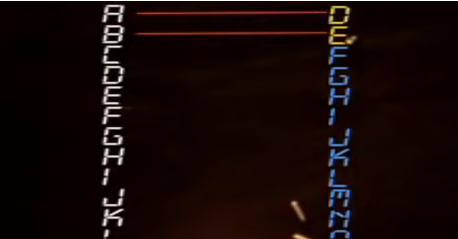
\includegraphics[scale=1]{1.png}
\end{center}
So A becomes D, B becomes E, C becomes F, and so on. This unreadable, or encrypted message, is then sent to Bob openly. Then Bob simply subtracts the shift of three from each letter in order to read the original message. Incredibly, this basic cipher was used by military leaders for hundreds of years after Caesar.
However, a lock is only as strong as its weakest point. A lock breaker may look for mechanical flaws. Or failing that, extract information in order to narrow down the correct combination. The process of lock breaking and code breaking are very similar. The weakness of the Caesar Cipher was published 800 years later by an Arab mathematician named Al-Kindi. He broke the Caesar Cipher by using a clue based on an important property of the language a message is written in.
If you scan text from any book and count the frequency of each letter, you will find a fairly consistent pattern.
\dfn{Frequency Table Of Letters}{A frequency table of letters, also known as a letter frequency distribution, displays how often each letter of the alphabet appears in a given text or dataset. Similar to a word frequency distribution, a letter frequency table provides insights into the usage patterns and prominence of different letters within the text.}
For example, these are the letter frequencies of English.This can be thought of as a fingerprint of English.

\begin{center}
	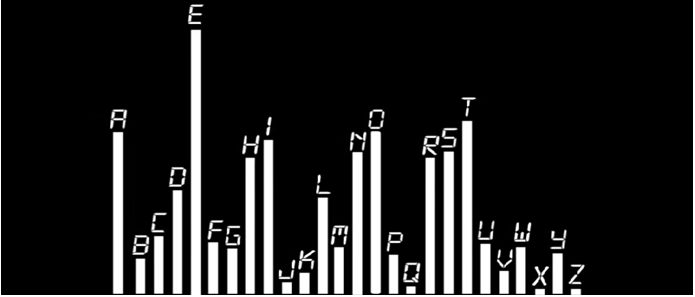
\includegraphics[scale=1]{2.png}
\end{center}
We leave this fingerprint when we communicate without realizing it. This clue is one of the most valuable tools for a codebreaker. To break this cipher, they count up the frequencies of each letter in the encrypted text and check how far the fingerprint has shifted.
\dfn{Frequency Analysis}{if H is the most popular letter in the encrypted message instead of E, then the shift was likely three. So they reverse the shift in order to reveal the original message. This is called frequency analysis, and it was a blow to the security of the Caesar cipher.}

\section{Polyalphabetic cipher}

A strong cipher is one which disguises your fingerprint. To make a lighter fingerprint is to flatten this distribution of letter frequencies. By the mid-15th century, we had advanced to polyalphabetic ciphers to accomplish this.
Imagine Alice and Bob shared a secret shift word. First, Alice converts the word into numbers according to the letter position in the alphabet. Next, this sequence of numbers is repeated along the message. Then each letter in the message is encrypted by shifting according to the number below it. 
\begin{center}
	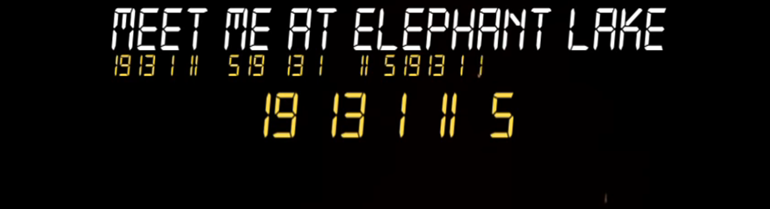
\includegraphics[scale=1]{3.png}
\end{center}
Now she is using multiple shifts instead of a single shift across the message, as Caesar had done before. Then the encrypted message is sent openly to Bob. Bob decrypts the message by subtracting the shifts according to the secret word he also has a copy of. 
Now imagine a code breaker, Eve, intercepts a series of messages and calculates the letter frequencies. She will find a flatter distribution, or a lighter fingerprint. So how could she break this? 
Remember, code breakers look for information leak, the same as finding a partial fingerprint. Any time there is a differential in letter frequencies, a leak of information occurs. This difference is caused by repetition in the encrypted message. In this case, Alice's cipher contains a repeating code word. To break the encryption, Even would first need to determine the length of this shift word used, not the word itself.
\begin{center}
	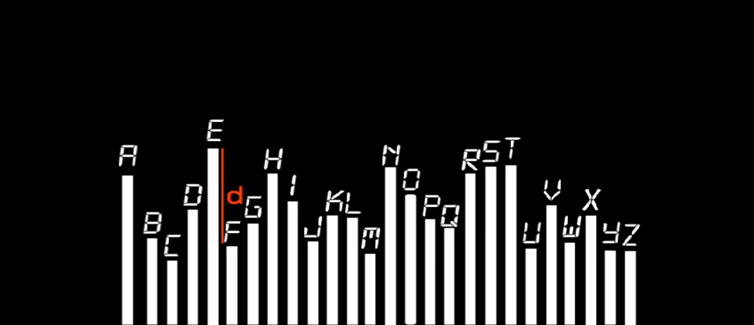
\includegraphics[scale=1]{4.png}
\end{center}
 She will need to go through and check the frequency distribution of different intervals. When she checks the frequency distribution of every fifth letter, the fingerprint will reveal itself. The problem now is to break five Cesar Ciphers in a repeating sequence. Individually this is a trivial task, as we have seen before. The added strength of this cipher is the time taken to determine the length of the shift word used. The longer the shift word, the stronger the cipher.
 
 \section{The one-time pad}
 
 For over 400 years, the problem remained. How could Alice design a cipher that hides her fingerprint, thus stopping the leak of information?
 The answer is randomness. Imagine Alice rolled a 26 sided die to generate a long list of random shifts, and shared this with Bob instead of a code word. Now, to encrypt her message, Alice uses the list of random shifts instead. It is important that this list of shifts be as long as the message, as to avoid any repetition. Then she sends it to Bob, who decrypts the message using the same list of random shifts she had given him.
 Now Eve will have a problem, because the resulting encrypted message will have two powerful properties. \\
 One, the shifts never fall into a repetitive pattern. And two, the encrypted message will have a \textbf{uniform frequency distribution}. Because there is no frequency differential and therefore no leak, it is now impossible for Eve to break the encryption. This is the strongest possible method of encryption, and it emerged towards the end of the 19th century. It is now known as the one-time pad. \\
 In order to visualize the strength of the one-time pad, we must understand the combinatorial explosion which takes place. For example, the Caesar Cipher shifted every letter by the same shift, which was some number between 1 and 26. So if Alice was to encrypt her name, it would result in one of 26 possible encryptions. \\
 A small number of possibilities, easy to check them all, known as brute force search. Compare this to the one-time pad, where each letter would be shifted by a different number between 1 and 26. Now think about the number of possible encryptions. It's going to be 26 multiplied by itself five times, which is almost 12 million.\\
 Sometimes it's hard to visualize, so imagine she wrote her name on a single page, and on top of it stacked every possible encryption. How high do you think this would be? With almost 12 million possible five-letter sequences, this stack of paper would be enormous, over one kilometer high.\\
 When Alice encrypts her name using the one-time pad, it is the same as picking one of these pages at random. From the perspective of Eve, the code breaker, every five letter encrypted word she has is equally likely to be any word in this stack. So this is perfect secrecy in action.
 
 \section{Frequency stability property short film}
 Consider the following. Imagine two rooms.\\
 Inside each room is a switch. In one room, there is a man who flips his switch according to a coin flip. If he lands heads, the switch is on. If he lands tails, the switch is off. In the other room, a woman switches her light based on a blind guess. She tries to simulate randomness without a coin. Then we start a clock, and they make their switches in unison. \\
 Can you determine which light bulb is being switched by a coin flip? The answer is yes, but how? \\
 And the trick is to think about properties of each sequence rather than looking for any specific patterns. For example, first, we may try to count the number of 1's and 0's which occur in each sequence. This is close, but not enough since they will both seem fairly even. The answer is to count sequences of numbers, such as runs of three consecutive switches. 
 \dfn{Frequency Stability Property}{A true random sequence will be equally likely to contain every sequence of any length.This is called the frequency stability property and is demonstrated by this uniform graph.\begin{center}
 		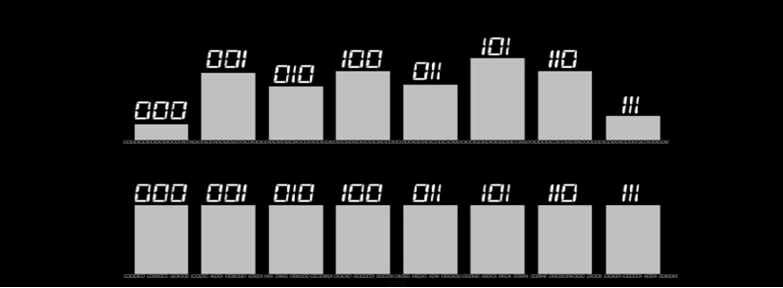
\includegraphics[scale=0.8]{5.png}
 	\end{center}
 	 }
  Humans favor certain sequences when they make guesses, resulting in uneven patterns such as we see here. One reason this happens is because we make the mistake of thinking certain outcomes are less random than others. But realize, there is no such thing as a lucky number. There is no such thing as a lucky sequence. \\
 If we flip a coin 10 times, it is equally likely to come up all heads, all tails, or any other sequence you can think of.
 
 \section{The Enigma encryption machine}
 
 On August 5th, 1857, a 4,300 kilometer-long cable was laid across the Atlantic Ocean. It provided a link between Britain and the Americas, further strengthening their social and economic alliances. Now information could be represented as a pattern of electrical pulses and sent across the world almost instantaneously. Stock tickers and money transfers - these were commercial applications invented by Western Union which ushered in a new era of global communication.\\
 During World War Two, Germany, Italy, and Japan were far outnumbered by the allies. Their only conceivable path to victory was the ability to launch widespread surprise attacks. So the goal of encryption technology was to automate the one-time pad using an encryption machine.\\
 Ideally, this machine would accept an input letter, apply a random shift, and output the encrypted letter. However, all machines follow the same principle. \\
 They begin in some initial configuration known as a state, they accept some input, they do an operation with the input, and then they produce an output. The operation from initial state to final state is always predictable and repeatable. So the goal was to produce identical machines that output a scrambled sequence of shifts, which took a long time to repeat.\\ 
 Therefore, Alice and Bob could generate an identical shift sequence as follows: First they need to share identical machines and agree on an initial position, which is defined as the key setting. Then they align their machines to the same position, and finally cycle through the identical operations to achieve identical sequences. Now the state-of-the-art technology at the time was called a rotor encryption machine. We are all familiar with the mechanical process of an odometer, which takes a long time to finally repeat its cycle. \\
 Now imagine we scramble the numbers on the wheels of the odometer. When it ticks forward, a new shift could be generated by adding up each number on the rotors.
 \begin{center}
 	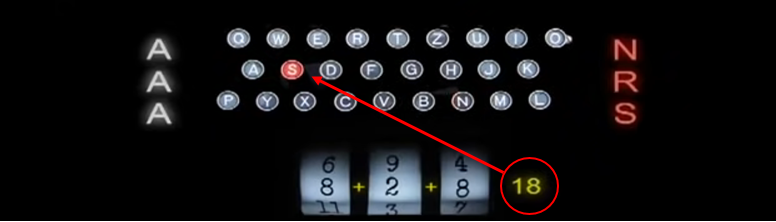
\includegraphics[scale=1]{6.png}
 \end{center}
This is the rough idea behind rotor encryption machines. For example, the message, "Attack Northwest" would be encrypted as follows.
  \begin{center}
 	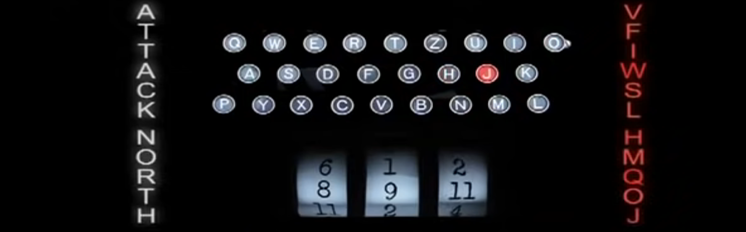
\includegraphics[scale=1]{7.png}
 \end{center}
 Notice how a new shift is used at each position in the message. With three rotors, each with 26 numbers, the length of the sequence before repeating is 26 times 26 times 26. This is equivalent to having a list of shifts 17,576 numbers long. Understand that each rotor position is equivalent to a location in this sequence. The initial machine state is known as the key setting, and the collection of all possible key settings defines the key space. This key space increases if the number of ways to initially configure the machine increases. For example, if the rotors can be rearranged then the order can be selected in six ways $3*2*1=6$.\\
Let's visualize the key space at this point. First we choose from one of six possible rotor orderings, then we select an initial position from the rotor sequence. This give us a key space with over 100,000 key settings. Remember, every machine configuration is a point in this space.\\ When we select a key setting, we are selecting a starting point in this space, which then determines the rest of the shift sequence. Give away the key setting and you give away the entire sequence.\\
The security of rotor machines depends on both the size of this key space and the randomness of the key setting. \\
During World War Two, one of the most important encryption technologies used by the German military was known as the Enigma. It was an eletro-mechanical rotor machine invented by a German engineer at the end of World War One. Each rotor wheel had electrical contacts on either side with a maze of wirings within. So at each rotor position, there was an electrical path from every input letter to every output letter. When the rotor advanced, an entirely new path was defined for each letter.
\begin{center}
	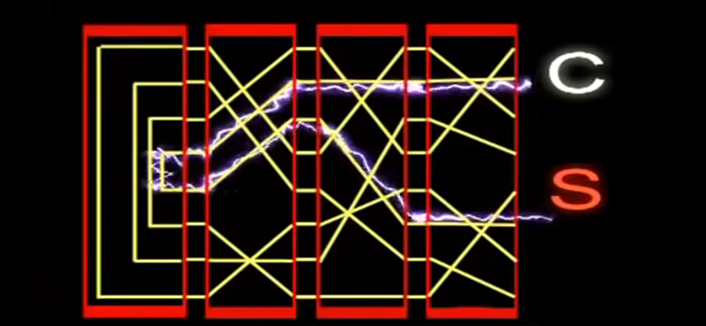
\includegraphics[scale=1]{8.png}
\end{center}
 During the war, they continually tried to increase the key space of the Enigma in order to make it stronger. For example, some changes they made were to add a fourth rotor wheel and increase the number of possible rotors you could put in the machine to 60. This had the effect of massively increasing the key space. Near the end of the war, the Enigma could be set up in over 150 million, million, million ways. Guessing the key setting which was used for a given message was about as likely as guessing the outcome of 26 dice rolls. This gave the Germans confidence that the Allies, even if they had a copy of the Enigma, could never check all possible key settings. For two parties to communicate using the Enigma, it required that they first shared the daily key settings. This allowed them to align their machines to the same position. This protocol changed over and over during the war, but generally involved distributing key sheets in advance to all operators. Each day, the operator would cut off the daily settings and this would tell them the daily configuration of their machines, such as what rotors to use and the order of the rotors. This key setting was then to be destroyed after use. However, one vital step was left to the operator. They were to select a random initial position of each rotor before communication began. And a very simple mistake was made by some fatigued operators. We make this exact same mistake every time we set a bike lock combination, because we tend to rotate the cylinders only a few clicks from the initial state, or we reuse a common password. This destroyed the uniform distribution of the initial rotor position, and after repeated observations, it allowed the Allies to reverse engineer the rotor wirings completely. The second major error was a design error, not a procedural one. \\
The Enigma was designed so that an input letter would never encrypt to itself. So given an encrypted letter, such as  'L', You can now eliminate the possibility that 'L' was the original letter. What they thought was a strength was actually a \underline{weakness} in design. \\
And this led to a code breaking machine, initially designed by the Poles and later improved by the British-American effort. The Bombe was multiple Enigma rotors chained together, allowing it to rapidly test different key settings. It took advantage of the fact that common words were known to be in the original message, such as weather. And these came to be known as cribs. For a given message in crib, the Bombe could scan through all possible rotor positions and orders in order to find possible key settings in a matter of minutes. This machine allowed the Allies to read German commands within hours of them being issued. It was a fatal blow to their combat strategy, as the Allies could anticipate their next move. \\
One fact remains: This initial attempt at automating the one-time pad failed. If the operators had instead rolled dice to decide their initial rotor positions, the starting point 

\section{Perfect secrecy}

Consider the following game.\\
Eve instructs Bob to go into a room. Bob finds the room empty, except for some locks, an empty box, and a single deck of cards. Eve tells Bob to select a card from the deck and hide it as best he can. \\
The rules are simple. Bob cannot leave the room with anything, cards and keys all stay in the room, and he can put, at most, one card in the box. Eve agrees that she has never seen the locks. He wins the game if Eve is unable to determine his card. So what is his best strategy?\\
Well, Bob selected a card, six of diamonds, and threw it in the box. First he considered the different types of locks. Maybe he should lock the card in the box with the key. Though, she could pick locks, so he considers the combination lock. The key is on the back, so if he locks it and scratches it off, it seems like the best choice. \\
\underline{But suddenly he realizes the problem}. The remaining cards on the table leak information about his choice, since it's now missing from the deck. The locks are a decoy. (metal jangles) He shouldn't separate his card from the deck. He returns his card to the deck but can't remember the position of his card. So he shuffles the deck to randomize it. Shuffling is the best lock, because it leaves no information about his choice. His card is now equally likely to be any card in the deck. He can now leave the cards openly, in confidence. Bob wins the game, because the best Eve can do is simply guess, as he has left no information about his choice. Most importantly, even if we give Eve unlimited computational power, she can't do any better than a guess. This defines what we call \textbf{perfect secrecy}.
\dfn{Perfect Secrecy}{Perfect Secrecy is a cryptographic property ensuring that even with unlimited computational power and access to auxiliary information, an eavesdropper gains no insight into a communicated message or secret, making decryption or inference impossible.
}
On September first, 1945, 29-year-old Claude Shannon published a classified paper on this idea. Shannon gave the first mathematical proof for how and why the one time pad is perfectly secret. Shannon thinks about encryption schemes in the following way. \\
Imagine Alice writes a message to Bob, 20 letters long. This is equivalent to picking one specific page from the message space. The message space can be thought of as a complete collection of all possible 20 letter messages. Anything you can think of that's 20 letters long is a page in this stack. Next, Alice applies a shared key, which is a list of 20 randomly generated shifts between one and 26. The key space is the complete collection of all possible outcomes, so generating a key is equivalent to selecting a page from this stack at random. When she applies the shift to encrypt the message, she ends up with a cipher text. The cipher text space represents all possible results of an encryption. When she applies the key, it maps to a unique page in this stack. \\
Notice that the size of the message space equals the size of the key space equals the size of the cipher text space. This defines what we call "perfect secrecy," for if someone has access to a page of cipher text only, the only thing that they know is that every message is equally likely. So no amount of computational power could ever help improve a blind guess. Now the big problem, you're wondering, with the time pad, is we have to share these long keys in advance.\\
To solve this problem, we need to relax our definition of secrecy by developing a definition of pseudo-randomness. 

\section{Pseudorandom number generators}

When we observe the physical world we find random fluctuations everywhere. We can generate truly random numbers by measuring random fluctuations, known as noise. When we measure this noise, known as sampling, we can obtain numbers. For example, if we measure the electric current of TV static over time, we will generate a truly random sequence. We can visualize this random sequence by drawing a path that changes direction according to each number, known as a \textbf{random walk}.
\dfn{Random Walk}{A random walk is a stochastic process that models the movement or progression of a point or entity in a sequence of discrete steps, where each step is determined by a random value obtained from measuring inherent random fluctuations or noise in a system. This process generates a path that exhibits unpredictable changes in direction, akin to the observed fluctuations in the physical world, such as the trajectory traced by a point subject to successive random deviations derived from measuring phenomena like electric current fluctuations in TV static.}
Notice the lack of pattern at all scales. At each point in the sequence the next move is always unpredictable. Random processes are said to be nondeterministic, since they are impossible to determine in advance. Machines, on the other hand, are deterministic. Their operation is predictable and repeatable.\\
In 1946, John von Neumann was involved in running computations for the military; specifically involved in the design of the hydrogen bomb. Using a computer called the ENIAC, he planned to repeatedly calculate approximations of the processes involved in nuclear fission. However, this required quick access to randomly generated numbers that could be repeated, if needed. However, the ENIAC had very limited internal memory; storing long random sequences was not possible. So, Neumann developed an algorithm to mechanically simulate the scrambling aspect of randomness as follows:\\
First, select a truly random number, called the \textbf{seed}. This number could come from the measurement of noise, or the current time in milliseconds. Next, this seed is provided as input to a simple calculation. Multiply the seed by itself, and then output the middle of this result. Then you use this output as the next seed, and repeat the process as many times as needed. This is known as the middle-squares method and is just the first in a long line of pseudorandom number generators. The randomness of the sequence is dependent on the randomness of the initial seed only. Same seed, same sequence. So, what are the differences between a randomly generated versus pseudorandomly generated sequence? Let's represent each sequence as a random walk. They seem similar until we speed things up. The pseudorandom sequence must eventually repeat. This occurs when the algorithm reaches a seed it has previously used, and the cycle repeats. The length, before a pseudorandom sequence repeats, is called \textbf{the period}.\\
 The period is strictly limited by the length of the initial seed. For example, if we use a two-digit seed, then an algorithm can produce, at most, 100 numbers, before reusing a seed and repeating the cycle. A three-digit seed can't expand past 1,000 numbers before repeating its cycle, and a four-digit seed can't expand past 10,000 numbers before repeating. Though if we use a seed large enough, the sequence can expand into trillions and trillions of digits before repeating. Though the key difference is important. When you generate numbers pseudorandomly, there are many sequences which cannot occur.\\
For example, if Alice generates a truly random sequence of 20 shifts, it's equivalent to a uniform selection from the stack of all possible sequences of shifts. This stack contains 26 to the power of 20 pages $\mathbf{26^{20}}$, which is astronomical in size. If we stood at the bottom and shined a light upwards, a person at the top would not see the light for around 200,000,000 years. Compare this to Alice generating a 20 digit pseudorandom sequence, using a four-digit random seed. Now, this is equivalent to a uniform selection from 10,000 possible initial seeds, meaning she can only generate 10,000 different sequences, which is a vanishingly small fraction of all possible sequences. When we move from random to pseudorandom shifts, we shrink the key space into a much, much smaller seed-space. So, for a pseudorandom sequence to be indistinguishable from a randomly generated sequence, it must be impractical for a computer to try all seeds and look for a match. This leads to an important distinction in computer science, between what is possible, versus what is possible in a reasonable amount of time. We use the same logic when we buy a bike lock. We know that anybody can simply try all possible combinations, until they find a match and it opens. But it would take them days to do so. So, for eight hours we assume it's practically safe.\\
With pseudorandom generators, the security increases as the length of the seed increases. If the most powerful computer would take hundreds of years to run through all seeds, then we safely can assume it's practically secure, instead of perfectly secure. As computers get faster the seed size must increase accordingly. Pseudorandomness frees Alice and Bob from having to share their entire random shift sequence in advance. Instead, they share a relatively short random seed, and expand it into the same random-looking sequence when needed. But what happens if they can never meet to share this random seed?
\newpage

\chapter{Ciphers}
\newpage
\section{Ciphers vs. codes}
To begin, let’s make sure we understand the difference between a cipher and a code. Actually, I dare you to get up and go ask someone the same question right now. While you do that I’ll wait here and admire this Lorenz cipher machine
\begin{center}
	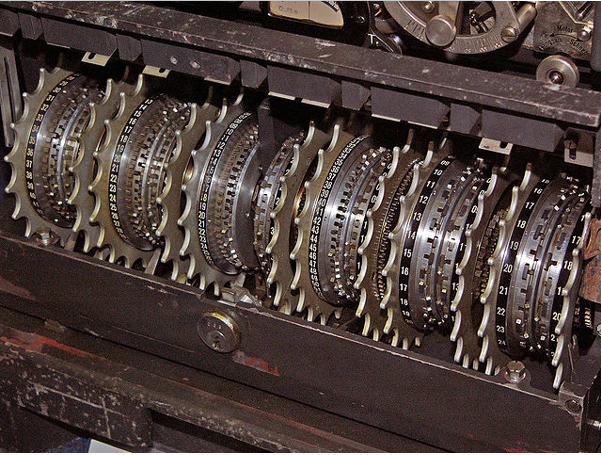
\includegraphics[scale=1]{9.png}
\end{center}Did they stumble around for an answer? For most people, it’s as if you asked them what the difference is between mix and blend. Tough question. Luckily, we have a video on  Morse Code which introduces the idea of a \textbf{codebook}
\begin{center}
	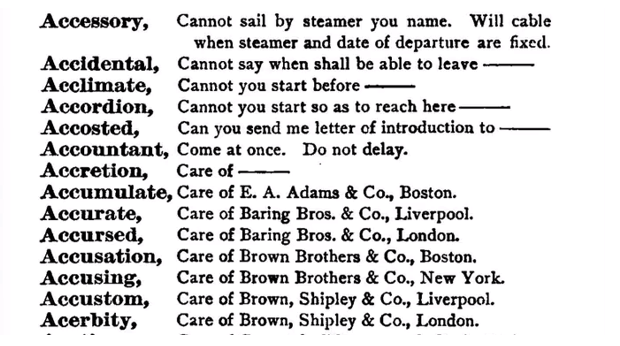
\includegraphics[scale=1]{10.png}
\end{center}Here, the word accountant is code for "Come at once. Do not delay." A code is a mapping from some meaningful unit—such as a word, sentence, or phrase— into something else—usually a shorter group of symbols. For example, we could make up a code where the word apple is written as 67. Generally codes are ways of saving time, and when sending messages around the world, time is money.\\
A codebook is simply a list of these mappings. Codebooks have been around ever since we began writing. Just remember, a code requires a codebook.
Okay, so what about ciphers?
Most importantly, ciphers do not involve meaning. Instead they are mechanical operations, known as algorithms, that are performed on individual or small chunks of letters. For example, in the Caesar Cipher we saw how each letter in the alphabet was mapped to a different letter. For example, A→D ,  B→E , and C→F , when we're using a shift of four. This kind of cipher is known as a \textbf{shift cipher}.\\
In this case, we don’t need a codebook. Instead, we follow a series of instructions—also known as an \textbf{algorithm}—where we shift each letter by a certain number. The algorithm requires one piece of shared information known as a \textbf{key}. In the example above where A→D, the key is four. This shared key is required for two parties to \textbf{encrypt} messages: HELLO → KHOOR, and \textbf{decrypt} messages: KHOOR→HELLO.\\
So back to our question: What is the difference between codes and ciphers? Codes generally operate on semantics, meaning, while ciphers operate on syntax, symbols. A code is stored as a mapping in a codebook, while ciphers transform individual symbols according to an algorithm.
\section{Shift cipher}
Now, let’s review the mechanics involved in the Caesar Cipher in the next exercise.
\dfn{Shift Cipher}{The Caesar Cipher is a type of shift cipher. Shift Ciphers work by using the modulo operator to encrypt and decrypt messages. The Shift Cipher has a key K, which is an integer from 0 to 25. We will only share this key with people that we want to see our message.}
\begin{algorithm}[H]
	\KwIn{original massage M}
	\KwOut{encrypted massage C}
	\SetAlgoLined
	\SetNoFillComment
	\tcc{For every letter in the message M:}
	\vspace{3mm}
	Convert the letter into the number that matches its order in the alphabet starting from 0, and call this number X.
	( A=0, B=1, C=2, ...,Y=24, Z=25)
	
	Calculate: Y = (X + K) mod 26
	
	Convert the number Y into a letter that matches its order in the alphabet starting from 0.
	(A=0, B=1, C=2, ...,Y=24, Z=25)
	
	\caption{How to Encrypt:}
\end{algorithm}

\begin{algorithm}[H]
	\KwIn{encrypted massage C}
	\KwOut{original massage M}
	\SetAlgoLined
	\SetNoFillComment
	\tcc{For every letter in the cipher text C:}
	\vspace{3mm}
	Convert the letter into the number that matches its order in the alphabet starting from 0, and call this number Y.
	(A=0, B=1, C=2, ..., Y=24, Z=25)
	
	
	Calculate: X= (Y - K) mod 26
	
	Convert the number X into a letter that matches its order in the alphabet starting from 0.
	(A=0, B=1, C=2, ..., Y=24, Z=25)
	
	
	\caption{How to Decrypt:}
\end{algorithm}

\subsection{Why is the Shift Cipher insecure?}
A cipher should prevent an attacker, who has a copy of the cipher text but does not know the key, from discovering the contents of the message.\textbf{ Since we only have 26 choices for the key}, someone can easily try all of the 26 keys, one by one, until they recover the message. This type of attack is called \textbf{a brute force attack}.

\section{XOR bitwise operation}
\subsection{The ultimate shift cipher}

If you’ve seen the lesson on the one-time pad, you know that it is \textbf{the ultimate shift cipher}. It involves the application of a random list of shifts equal to the length of the message. It’s important to understand exactly how and why the one-time pad is unbreakable, or, perfectly secret.\\
To understand why, we need to first introduce the \textbf{AND}, \textbf{OR} and \textbf{XOR} bitwise operations. Specifically why XOR must be used when performing the one-time pad on computers. \textbf{Bitwise} simply means that we are dealing with individual bits, or binary numbers. In any modern/computerized encryption scheme we represent our symbols using binary digits. 

\subsection{Encrypting Colors}
Let’s begin with a visual example by \textbf{encrypting the color} of the Khan Academy green leaf avatar.\\
How do we turn a color into a number? Well, right now you are looking at HTML colors which are defined using the \textbf{RGB color model}. This is an additive model based on mixing some amount of \textbf{red, green and blue light}.
\begin{center}
	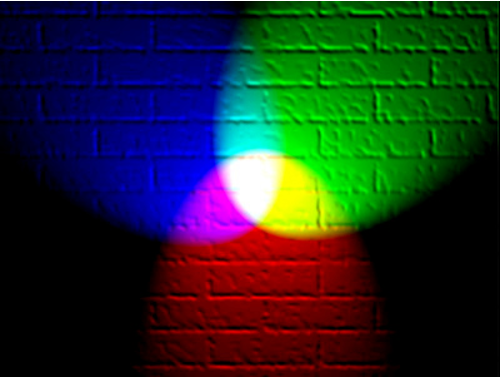
\includegraphics[scale=1]{11.png}
\end{center}We can define exactly how much RED, GREEN and BLUE using a number from 0-255. Black is all off (0,0,0) while white is all on (255,255,255). In between there are \textbf{16 million possible colors} (256 * 256 * 256).
\newpage
\ex{Green Sample}{
\begin{center}
	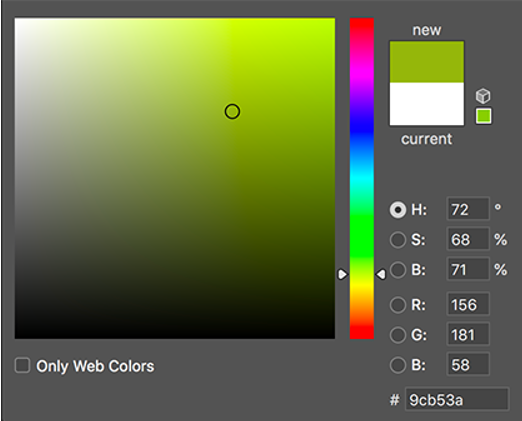
\includegraphics[scale=1]{12.png}
	
	\textbf{Figure 1:}Screenshot of the Photoshop color picker, with green selected.
\end{center}
RED=156 \quad $\rightarrow$ \quad RED=10011100

GREEN=181 \quad $\rightarrow$ \quad GREEN=10110101

BLUE=58 \quad $\rightarrow$ \quad BLUE=00111010

We can squeeze those together as: 100111001011010100111010

\begin{center}
	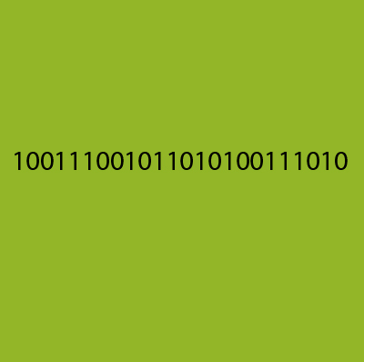
\includegraphics[scale=1]{13.png}
	
	\textbf{Figure 2:} Green background with 100111001011010100111010 on top
	
\end{center}
}

\subsection{Application of random shifts}

Now let’s say you generate a shift sequence using coin flips converted into binary as:\\
\textbf{HTHTTHTHHHHTTHTTTTHTTHHH = 010110100001101111011000}\\
Let’s think about how we could apply this shift sequence to our color in order to encrypt it using the one-time pad:\\
\textbf{100111001011010100111010 + 010110100001101111011000 = ??}\\
To make the one-time pad work we need to choose the correct operation so that the resulting sequence is equally likely to be any color. Let’s go over three different operations, \textbf{AND, OR, XOR}.

\subsection{AND}

The AND operator is also known as logical conjunction, and works just like multiplication. 
It outputs a 1 only if all of the inputs are 1. . Here is the truth table:\\
0 AND 0 = 0\\
0 AND 1 = 0\\
1 AND 0 = 0\\
1 AND 1 = 1\\
\ex{}{100111001011010100111010 AND 010110100001101111011000 = 000110000001000100011000
\begin{center}
	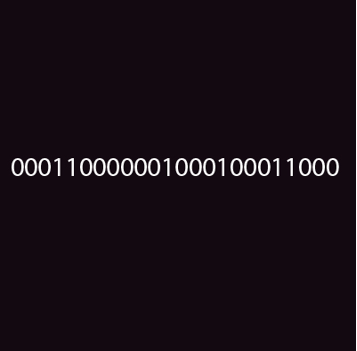
\includegraphics[scale=1]{14.png}
\end{center}

This results in a very dark purple. Notice when we perform the AND operation on any binary number, the resulting sequence cannot be larger. In our color example this eliminates many possible shades as it pushes the color \textbf{towards black}.
}

\newpage
\subsection{OR}
The OR operator is also known as logical disjunction. It outputs a 1 whenever one or more of its inputs are 1. Here is the truth table:\\
0 OR 0 = 0\\
0 OR 1 = 1\\
1 OR 0 = 1\\
1 OR 1 = 1\\
\ex{}{100111001011010100111010 OR 010110100001101111011000 = 110111101011111111111010

\begin{center}
	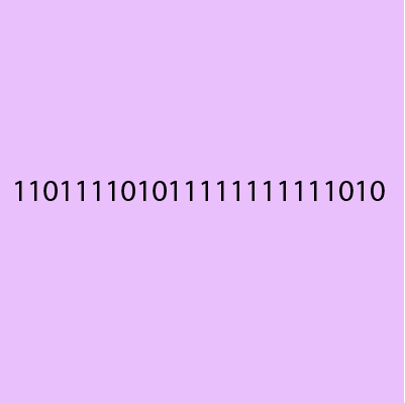
\includegraphics[scale=1]{15.png}
\end{center}

This results in a light purple. Notice when we perform the OR operation on any binary sequence, the resulting sequence cannot be smaller. This eliminates many possibilities as it pushes the color \textbf{towards white}.
}

\newpage
\subsection{XOR}

The XOR operator outputs a 1 whenever the inputs do not match, which occurs when one of the two inputs is exclusively true. This is the same as addition mod 2. Here is the truth table:\\
0 XOR 0 = 0\\
0 XOR 1 = 1\\
1 XOR 0 = 1\\
1 XOR 1 = 0\\
\ex{}{100111001011010100111010 XOR 010110100001101111011000 = 110001101010111011100010

\begin{center}
	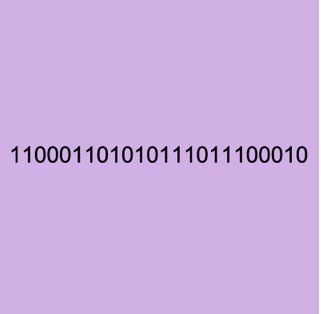
\includegraphics[scale=1]{16.png}
\end{center}

This results in a slightly darker purple as compared to the OR operation. Notice when we perform the XOR operation on a binary sequence, the resulting sequence could be any possible sequence. Given some encrypted color, all we know is the original color is "equally likely to be any color". We have no information that could improve a blind guess (1/16 million).
Finally, let’s do a visual demonstration so that we can see the one-time pad in action. Then we can earn more energy points!

}
\newpage

\section{XOR and the one-time pad}

\subsection{Why must we use XOR?}
Does it really matter if we used AND, OR or XOR with the one-time pad? The answer is yes, and it’s extremely important to understand why. Recall from the previous article that AND has a 75\% chance of outputting 0 and a 25\% chance of outputting a 1. While OR has a 25\% chance of outputting 0 and 75\% chance of outputting 1. While the XOR operation has a 50\% chance of outputting 0 or 1.

\ex{visual example to see the different scrambling effects of AND vs. OR vs. XOR  by encrypting an image}{
Here is a digital image of Charles Babbage:
\begin{center}
	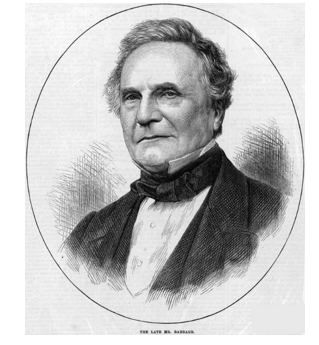
\includegraphics[scale=1]{17.png}
\end{center}
It contains thousands of tiny colored squares called pixels. Each pixel in this image can be represented as a 24 bit sequence as shown in the previous article. Let's call this our plaintext image (or message).
First let’s see what happens when we AND each bit in the image file with a stream of random bits.

\textbf{AND:}\\
Notice most of the original message shines through. This happens anytime a random shift of 1 is applied, or when the plaintext is 0:
\begin{center}
	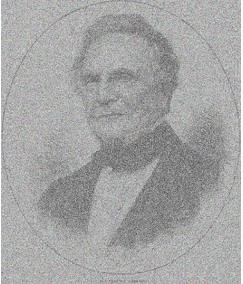
\includegraphics[scale=1]{18.png}
\end{center}
Next let’s see what happens when we OR each bit in the image file with a stream of random bits.

\textbf{OR:}\\
Notice most of the original message shines through. This happens anytime a random shift of 0 is applied, or when the plaintext is 1:
\begin{center}
	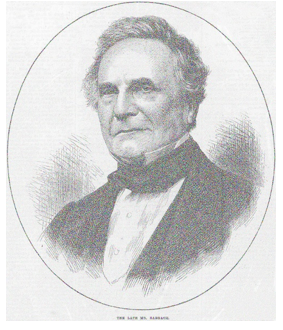
\includegraphics[scale=1]{19.png}
\end{center}
Finally, let’s see what happens when we XOR each bit in the image file with a stream of random bits.

\textbf{XOR:}
\begin{center}
	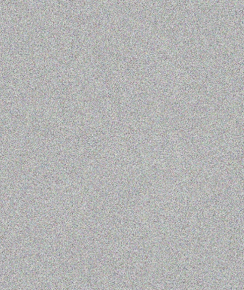
\includegraphics[scale=1]{20.png}
\end{center}
Where did Charles go?\\
Notice that the plaintext only shines through 50\% of the time, which results in noise as each pixel is equally likely to be 0 or 1.\\
This image contains no information about the original image. If we didn’t provide the shift sequence it would be impossible for you to reverse it back to the original image. You could try every possible sequence, but that would result in every possible image! How could you know it was Babbage? It's equally likely to be a picture of you or anything else you can think of.


}

\chapter{Modern cryptography }
\newpage
\section{The fundamental theorem of arithmetic}

Imagine we are living in prehistoric times. Now, consider the following. How did we keep track of time without a clock? All clocks are based on some repetitive pattern which divides the flow of time into equal segments. To find these repetitive patterns, we look towards the heavens. The sun rising and falling each day is the most obvious. However, to keep track of longer periods of time, we looked for longer cycles. For this we looked to the moon, which seemed to gradually grow and shrink over many days. When we count the number of days between full moons, we arrive at the number 29. This is the origin of a month. However, if we try to divide 29 into equal pieces, we run into a problem. It is impossible. The only way to divide 29 into equal pieces is to break it back down into single units. 29 is a prime number. Think of it as unbreakable. \\
If a number can be broken down into equal pieces greater than one, we call it a composite number. Now, if we are curious, we may wonder how many prime numbers are there, and how big do they get? Let's start by dividing all numbers into two categories. We list the primes on the left, and the composites on the right. At first they seem to dance back and forth. There is no obvious pattern here. So let's use a modern technique to see the big picture. 
\begin{center}
	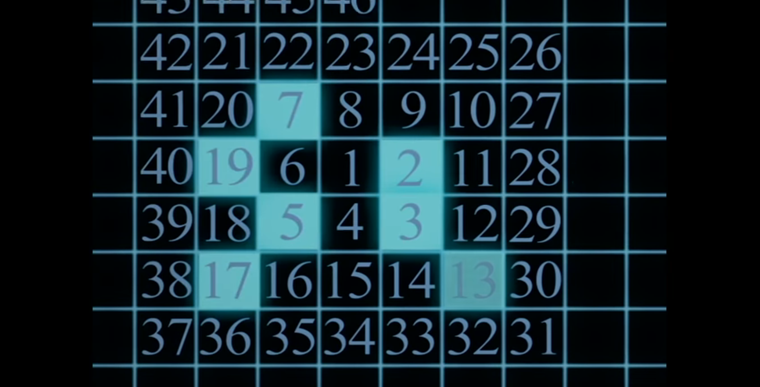
\includegraphics[scale=1]{21.png}
\end{center}
The trick is to use a Ulam spiral. First we list all possible numbers in order in a growing spiral. Then we color all the prime numbers blue. Finally, we zoom out to see millions of numbers. This is the pattern of primes, which goes on and on forever. Incredibly, the entire structure of this pattern is still unsolved today. We are on to something.\\
So let's fast forward to around 300 BC in ancient Greece. A philosopher known as Euclid of Alexandria understood that all numbers could be split into these two distinct categories. He began by realizing that any number can be divided down over and over until you reach a group of smallest equal numbers. And by definition, these smallest numbers are always prime numbers. So he knew that all numbers are somehow built out of smaller primes. To be clear, imagine the universe of all numbers, and ignore the primes. Now, pick any composite number and break it down, and you are always left with prime numbers. So Euclid knew that every number could be expressed using a group of smaller primes. Think of these as building blocks. No matter what number you choose, it can always be built with an addition of smaller primes. 
\begin{center}
	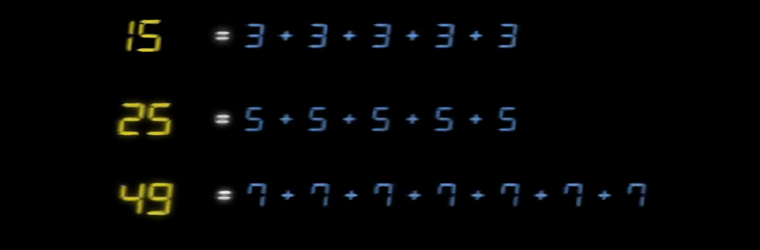
\includegraphics[scale=1]{22.png}
\end{center}
This is the root of his discovery, known as the fundamental theorem of arithmetic, as follows. Take any number, say 30, and find all the prime numbers it divides into equally. This we know as factorization. This will give us the prime factors.
\begin{center}
	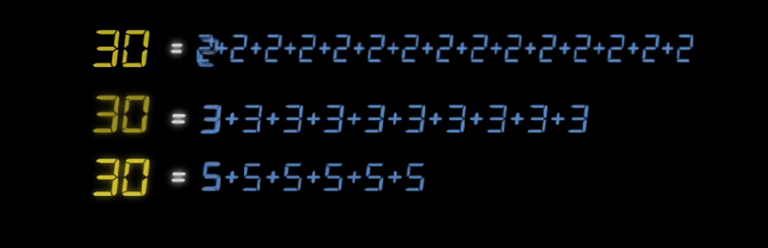
\includegraphics[scale=1]{23.png}
\end{center}
 In this case, 2, 3, and 5 are the prime factors of 30. Euclid realized that you could then multiply these prime factors a specific number of times to build the original number. In this case, you simply multiply each factor once to build 30. 2 times 3 times 5 is the prime factorization of 30. Think of it as a special key, or combination. There is no other way to build 30 using some other groups of prime numbers multiplied together. So every possible number has one, and only one prime factorization. A good analogy is to imagine each number as a different lock. The unique key for each lock would be its prime factorization. No two locks share a key. No two numbers share a prime factorization.

\section{Public key cryptography: What is it?}

After World War 2, with most of Europe in ruins, tension grew between the Soviet Union and the United States. It was clear that the next global superpower required the ability to both launch and successively defend nuclear attacks from intercontinental ballistic missiles. In North America, the most vulnerable point of attack was over the North Pole. So in 1958, a joint effort between United States and Canada was established, known as NORAD, or North American Aerospace Defense Command. An important line of defense was the semi-automatic ground environment. It was an automated system of over 100 long-distance radars scattered across North America. They were connected to computerized radar stations that transmitted tracking data using telephone lines or radio waves. All of this radar information was fed into a primary warning center buried a mile deep inside Cheyenne Mountain in Colorado. This application of machine to machine communication allowed operators to make split-second decisions using information transmitted and processed automatically by computers. This idea of being online was quickly adapted and advanced by universities in the following years as they understood the potential of computer networking.\\
Money transfers are just one of a growing number of applications which required encryption to remain secure; and as the internet grew to encompass millions around the world, a new problem emerged. At the time, encryption required two parties to first share a secret random number, known as a key. So how could two people who have never met agree on a secret shared key without letting Eve, who is always listening, also obtain a copy? \\
In 1976, Whitfield Diffie \& Martin Hellman devised an amazing trick to do this. First, let's explore how this trick is done using colors.  
\ex{How could Alice and Bob agree on a secret color without Eve finding it out?}{The trick is based on two facts: one, it's easy to mix two colors together to make a third color; and two, given a mixed color, it's hard to reverse it in order to find the exact original colors. This is the basis for a lock: easy in one direction, hard in the reverse direction.
	\begin{center}
		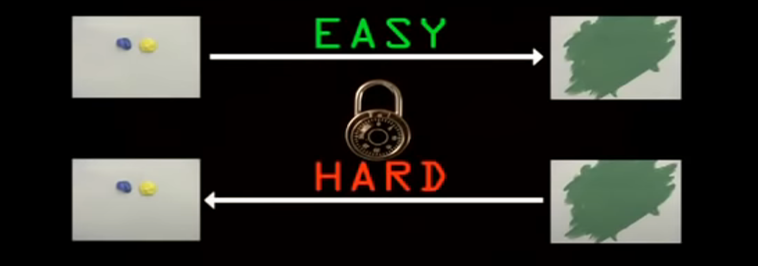
\includegraphics[scale=1]{24.png}
	\end{center}
	This is known as a one-way function. Now, the solution works as follows: First, they agree publicly on a starting color, say yellow. Next, Alice and Bob both randomly select private colors, and mix them into the public yellow in order to disguise their private colors. Now, Alice keeps her private color and sends her mixture to Bob, and Bob keeps his private color and sends his mixture to Alice.
	\begin{center}
		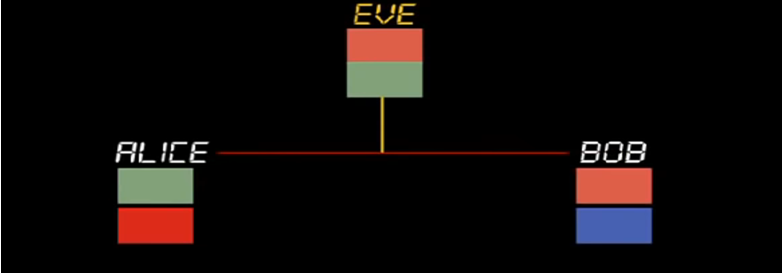
\includegraphics[scale=1]{25.png}
	\end{center}
	Now, the heart of the trick: Alice and Bob add their private colors to the other person's mixture and arrive at a shared secret color. Notice how Eve is unable to determine this exact color, since she needs one of their private colors to do so. And that is the trick. Now, to do this with numbers, we need a numerical procedure which is easy in one direction and hard in the other.}


\section{The discrete logarithm problem}

We need a numerical procedure, which is easy in one direction and hard in the other. This brings us to modular arithmetic, also known as clock arithmetic. For example, to find 46 mod 12, we could take a rope of length 46 units and rap it around a clock of 12 units, which is called the modulus, and where the rope ends is the solution. So we say 46 mod 12 is congruent to 10, easy. Now, to make this work, we use a prime modulus, such as 17, then we find a primitive root of 17, in this case three, which has this important property that when raised to different exponents, the solution distributes uniformly around the clock. Three is known as the generator. If we raise three to any exponent x, then the solution is equally likely to be any integer between zero and 17.
\begin{center}
	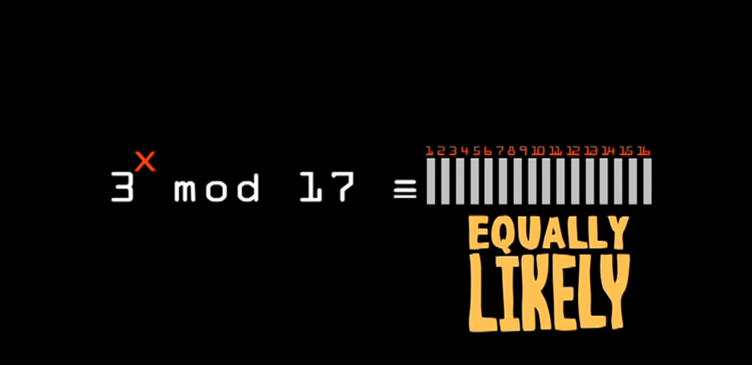
\includegraphics[scale=1]{26.png}
\end{center}
Now, the reverse procedure is hard. Say, given 12, find the exponent three needs to be raised to. This is called the\textbf{ discrete logarithm problem}.
\dfn{Discrete Logarithm Problem}{The discrete logarithm problem involves finding the exponent that, when applied to a given base element, results in a specific outcome within a finite cyclic group. It serves as a core challenge in number theory and cryptography, forming the basis for secure protocols like Diffie-Hellman key exchange and digital signatures. The problem's complexity underpins the security of these systems by making it computationally hard to solve efficiently, ensuring protection for sensitive information and communication.}
And now we have our one-way function, easy to perform but hard to reverse. Given 12, we would have to resort to trial and error to find matching exponents. 
\begin{center}
	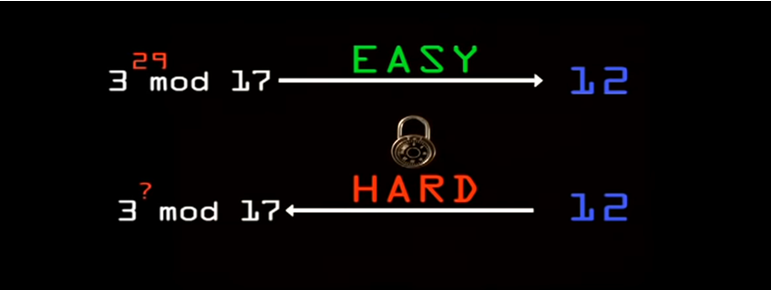
\includegraphics[scale=1]{27.png}
\end{center}
How hard is this? With small numbers it's easy, but if we use a prime modulus which is hundreds of digits long, it becomes impractical to solve. Even if you had access to all computational power on Earth, it could take thousands of years to run through all possibilities. So the strength of a one-way function is based on the time needed to reverse it.
\section{Diffie-hellman key exchange}
Now, this is our solution. First, Alice and Bob agree publicly on a prime modulus and a generator, in this case, 17 and three. Then, Alice selects a private, random number, say 15, and calculates$3^{15} \equiv 6^{17}$ , and sends this result publicly to Bob. Then Bob selects his private, random number, say 13, and calculates $3^{13} \equiv 12^{17}$ and sends this result publicly to Alice.\\ 
And now, the heart of the trick. Alice takes Bob's public result and raises it to the power of her private number to obtain the shared secret $12^{15} \equiv 10^{17}$, which in this case is 10. Bob takes Alice's public result and raises it to the power of his private number, resulting in the same shared secret $6^{13} \equiv 10^{17}$.\\
Notice they did the same calculation, though it may not look like it, at first. Consider Alice, the 12 she received from Bob was calculated as three to the power 13, mod 17. So her calculation was the same as three to the power 13, to the power 15, mod 17. Now consider Bob, the six he received from Alice was calculated as three to the power 15, mod 17. So his calculation was the same as three to the power 15, to the power 13. Notice they did the same calculation with the exponents in a different order. When you flip the exponent, the result doesn't change. So they both calculated three raised to the power of their private numbers. Without one of these private numbers, 15 or 13, Eve will not be able to find the solution. And this is how it's done. While Eve is stuck grinding away at the discrete logorithm problem, and with large enough numbers, we can say it's practically impossible for her to break the encryption in a reasonable amount of time. \\
This solves the key exchange problem. It can be used in conjunction with a pseudorandom generator to encrypt messages between people who have never met.

\section{RSA encryption}
\subsection{Step 1}
Up until the 1970s, cryptography had been based on symmetric keys. That is, the sender encrypts their message using a specific key, and the receiver decrypts using an identical key. \\
As you may recall, encryption is a mapping from some message using a specific key, to a ciphertext message. To decrypt a ciphertext, you use the same key to reverse the mapping. So for Alice and Bob to communicate securely, they must first share identical keys. However, establishing a shared key is often impossible if Alice and Bob can't physically meet or requires extra communications overhead when using the Diffy-Hellman key exchange. Plus, if Alice needs to communicate with multiple people, perhaps she's a bank, then she's going to have exchange distinct keys with each person. 
\begin{center}
	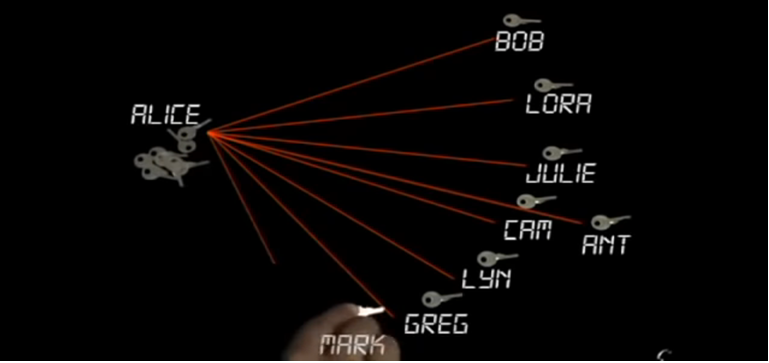
\includegraphics[scale=1]{28.png}
\end{center}
Now she'll have to manage all of these keys and send thousands of messages just to establish them. Could there be a simpler way? \\
In 1970, James Ellis, a British engineer and mathematician, was working on an idea for \textbf{non-secret encryption} . It's based on a simple, yet clever concept: Lock and unlock are inverse operations. Alice could buy a lock, keep the key, and send the open lock to Bob. Bob then locks his message and sends it back to Alice. No keys are exchanged. This means she could publish the lock widely and let anyone in the world use it to send her a message. And she now only needs to keep track of a single key.
\begin{center}
	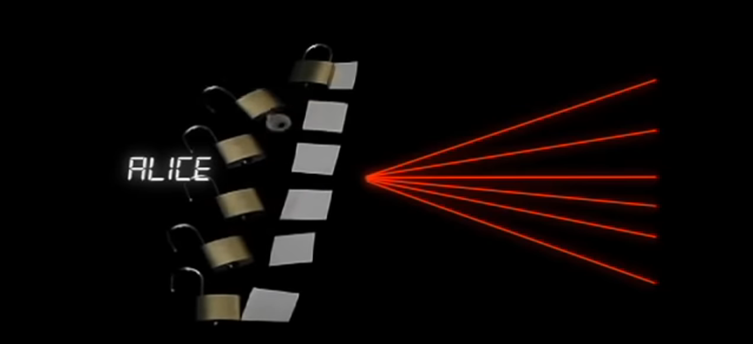
\includegraphics[scale=1]{29.png}
\end{center}
 Ellis never arrived at a mathematical solution, though he had an intuitive sense of how it should work. The idea is based on splitting a key into two parts, an encryption key and a decryption key. The decryption key performs the inverse or undo operation which was applied by the encryption key. \\
To see how inverse keys could work, let's do a simplified exampled with colors. How could Bob send Alice a specific color, without Eve, who is always listening, intercepting it? The inverse of some color is called a complimentary color, which when added to it, produces white, undoing the effect of the first color. 
\begin{center}
	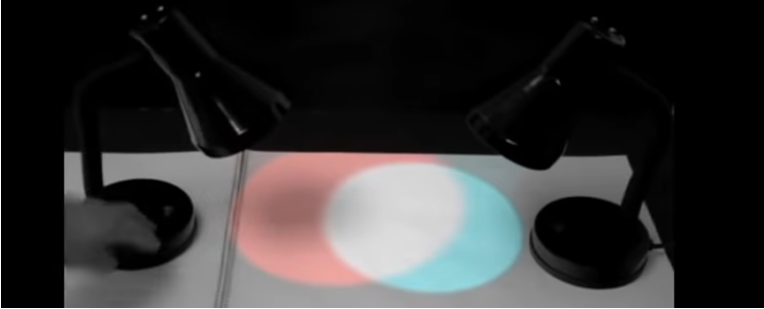
\includegraphics[scale=1]{30.png}
\end{center}
In this example, we assume that mixing colors is a one-way function because it's fast to mix colors and output a third, and it's much slower to undo. Alice first generates her private key by randomly selecting a color, say red. Next, assume Alice uses a secret color machine to find the exact compliment of her red and nobody else has access to this. This results in cyan, which she sends to Bob as her public key. Let's say Bob wants to send a secret yellow to Alice. He mixes this with her public color and sends the resulting mixture back to Alice. Now Alice adds her private color to Bob's mixture. This undoes the effect of her public color, leaving her with Bob's secret color. Notice Eve has no easy way to find Bob's yellow, since she needs Alice's private red to do so.
\begin{center}
	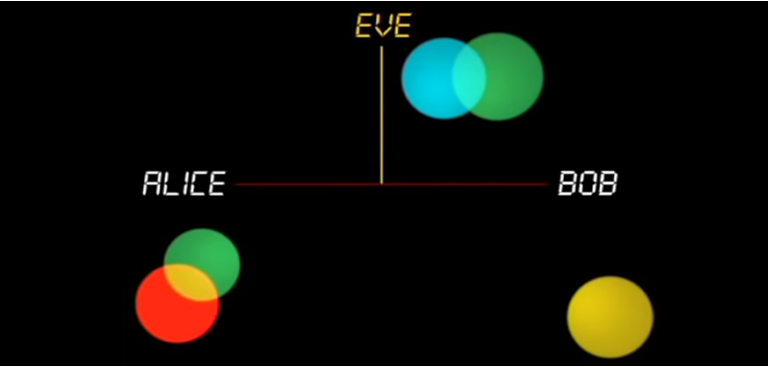
\includegraphics[scale=1]{31.png}
\end{center}
 This is how it should work. However, a mathematical solution was needed to make this work in practice.
\subsection{Step 2}
The solution was found by another British mathematician and cryptographer, Clifford Cocks. Cocks needed to construct a special kind of one-way function called \textbf{a trapdoor one-way function}. This is a function that is easy to compute in one direction, yet difficult to reverse, unless you have special information, called the \textbf{trapdoor}.\\
For this, he turned to modular exponentiation, which we introduced as clock arithmetic, in the Diffie–Hellman key exchange, as follows. Take a number, raise it to some exponent, divide by the modulus and output the remainder. This can be used to encrypt a message as follows: \\
Imagine Bob has a message, which is converted into a number, m. He then multiplies his number by itself, e times, where e is a public exponent, then he divides the result by a random number, N, and outputs the remainder of the division. This results in some number, c. This calculation is easy to perform, however, given only c, e, and N, it is much more difficult to determine which m was used, because we'd have to resort to some form of trial and error. 
\begin{center}
	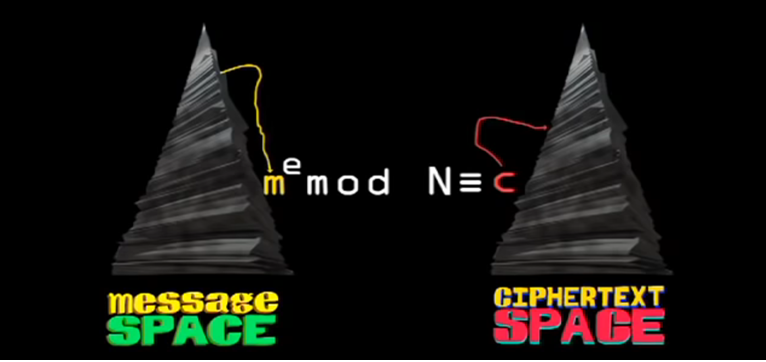
\includegraphics[scale=1]{32.png}
\end{center}
So, this is our one-way function that we can apply to m, easy to perform, but difficult to reverse. It is our mathematical lock. Now, what about the key? The key is the trapdoor, some piece of information that makes it easy to reverse the encryption. We need to raise c to some other exponent, say d, which will undo the initial operation applied to m and return the original message m.
$$m^e \text{mod N} \equiv c$$
$$c^{\color{blue}d} \text{mod N} \equiv m$$
 So, both operations together, is the same as m to the power of e, all raised to the power of d, which is the same as, m to the power of e times d, e is the encryption, d is the decryption.

$$m^{e^{\color{blue}d}} \text{mod N} \equiv m \quad \Rightarrow \quad m^{e\color{blue}d} \text{mod N} \equiv m$$
Therefore, we need a way for Alice to construct e and d, which makes it difficult for anyone else to find d This requires a second one-way function which is used for generating d, and for this, he looked back to Euclid.

\thm{}{
if $m^e \text{mod N} \equiv c$ and $c^{d} \text{mod N} \equiv m$ so we have:

$$m^{ed} \text{mod N} \equiv m$$
}

\subsection{Step 3}

Over 2,000 years ago, Euclid showed every number has exactly one prime factorization, which we can think of as a secret key. It turns out that prime factorization is a fundamentally hard problem. Let's clarify what we mean by "easy" and "hard", by introducing what's called "time complexity". \\
We have all multiplied numbers before, and each of us our own rules for doing so, in order to speed things up. If we program a computer to multiply numbers, it can do so much faster than any human can. Here is a graph that shows the time required for a computer to multiply two numbers. And, of course, the time required to find the answer increases as the numbers get larger. Notice that the computation time stays well under one second, even with fairly large numbers. Therefore, it is "easy" to perform. Now, compare this to prime factorization. If someone told you to find the prime factorization of 589, you will notice the problem feels harder. No matter what your strategy, it will require some trial and error until you find a number which evenly divides 589. After some struggle, you will find 19 times 31 is the prime factorization. If you were told to find the prime factorization of 437, 231, you'd probably give up and get a computer to help you. This works fine for small numbers, though if we try to get a computer to factor larger and larger numbers, there is a runaway effect. The time needed to perform the calculations increases rapidly, as there are more steps involved. As the numbers grow, the computer needs minutes, then hours, and eventually it will require hundreds, or thousands of years to factor huge numbers.
\begin{center}
	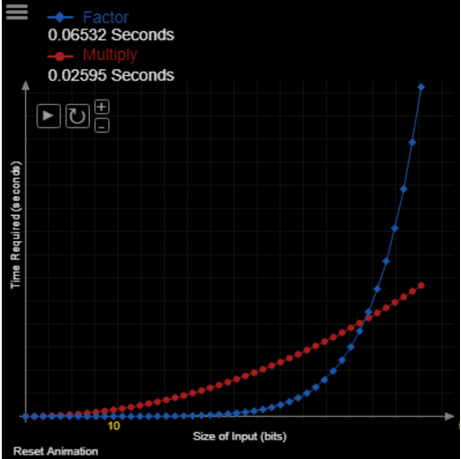
\includegraphics[scale=0.8]{36.png}
\end{center}
We therefore say it is a "hard" problem due to this growth rate of time needed to solve it. So factorization is what Cocks used to build the trapdoor solution.\\
Step one, imagine Alice randomly generated a prime number over 150 digits long; call this $\mathbf{P_1}$. Then, a second random prime number roughly the same size; call this $\mathbf{P_2}$. She then multiplies these two primes together to get a composite number, N, which is over 300 digits long.\\
This multiplication step would take less than second; we could even do it in a web browser. Then, she takes the factorization of N, p one times p two, and hides it. Now, if she gave N to anyone else, they would have to have a computer running for years to find the solution. \\
Step two, Cocks needed to find a function which depends on knowing the factorization of N. For this, he looked back to work done in 1760 by Swiss mathematician, Leonhard Euler.

\subsection{Euler's totient function}

Euler continued to investigate properties of numbers, specifically the distribution of prime numbers. One important function he defined is called the \textbf{phi function}. 
\dfn{Euler's Phi $(\phi)$ Function}{The Euler's Phi $(\phi)$ function, also known as the Euler totient function, is a mathematical concept used to compute the count of positive integers that are coprime (relatively prime) to a given positive integer n. In other words, it calculates the number of positive integers less than n that do not share any common factors with n, except for 1.
\\

formally, the Euler's Phi function is denoted as $\phi(n)$ and defined as follows:
\\

$\phi(n)$=count of integers 1$\leq$k$<$n such that gcd(n,k)=1
\\

Where:
\\

$\phi(n)$ represents the Euler's Phi function of n.

gcd(n,k) denotes the greatest common divisor of n and k.

} So, given a number, say N, it outputs how many integers are less than or equal to N that do not share any common factor with N. For example, if we want to find the $\phi(8)$ we look at all values from one to eight, then we count how many integers eight does not share a factor greater than one with. Notice six is not counted, because it shares a factor of two, while one, three, five and seven are all counted, because they only share a factor of one. Therefore,$\phi(8)$ equals four. What's interesting is that calculating the phi function is hard, except in one case.\ex{}{Given a number, say N, it outputs how many integers are less than or equal to N that do not share any common factor with N. For example, if we want to find the $\phi(8)$ we look at all values from one to eight, then we count how many integers eight does not share a factor greater than one with. Notice six is not counted, because it shares a factor of two, while one, three, five and seven are all counted, because they only share a factor of one. Therefore,$\phi(8)$ equals four.}
\newpage
What's interesting is that calculating the phi function is hard, except in one case. \\
Look at this graph. 
\begin{center}
	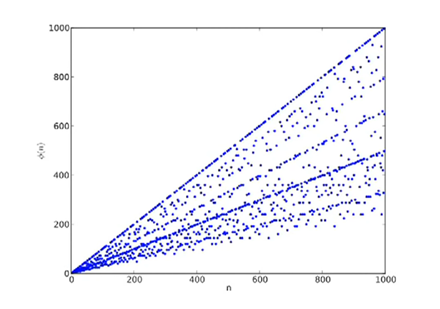
\includegraphics[scale=1]{37.png}
\end{center}
It is a plot of values of phi, over integers from one to 1,000. Now, notice any predictable pattern? The straight line of points along the top represent all the prime numbers. Since prime numbers have no factors greater than one, the phi of any prime number, P,   $\phi$($P$)=$P-1$  . To calculate phi of seven, a prime number, we count all integers, except seven, since none of them share a factor with seven. Phi of seven equals six. So, if you're asked to find phi of 21,377, a prime number, you would only need to subtract one to get the solution, 21,376. \\
Phi of any prime is easy to compute. This leads to an interesting result based on the fact that the phi function is also multiplicative. That is,   $\phi$($A$×$B$)=$\phi$($A$)×$\phi$($B$).
\begin{center}
	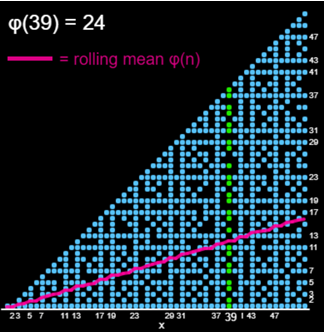
\includegraphics[scale=1]{38.png}
\end{center}
\thm{}{If we know some number N is the product of two primes, $P_1$ and $P_2$, then phi of N is just the value of phi for each prime multiplied together.\\
	$$\phi(N)=(P_1-1)*(P_2-1)$$.}

\newpage
\subsection{Step 4}
We now have a trapdoor for solving phi. If you know the factorization for N, then finding phi N is easy. For example, the prime factorization of 77 is 7×11, so phi of 77, is 6×10=60 \\
Step three, how to connect the phi function to modular exponentiation. For this, he turned to Euler's Theorem, which is a relationship between the phi function and modular exponentiation, as follows: 
$$m^{\phi(n)} \quad \equiv \quad \textcolor{red}{1}\quad \text{mod}\quad n$$
 This means you can pick any two numbers, such that they do not share a common factor, let's call them "m" and "n". Say m equals five and n equals eight. Now, when you raise m to the power of phi n, or 4, and divide by n, you will always be left with one.
\ex{}{$5^{\phi(8)}=625 \quad \equiv \quad  1\quad \text{mod}\quad 8$

m=5

n=8}
 Now, we just need to modify this equation using two simple rules.\\
First, if you raise the number one to any exponent, k, you always get one. In the same way, we can multiply the exponent phi n by any number k, and the solution is still one
$$1^k=1 \quad \Rightarrow \quad m^{k*\phi(n)} \quad \equiv \quad \textcolor{red}{1}\quad \text{mod}\quad n$$
Second, if you multiply one by any number, say m, it always equals m. In the same way, we can multiply the left side by m, to get m on the right hand side.
$$1*m=m \quad \Rightarrow \quad m*m^{k*\phi(n)} \quad \equiv \quad \textcolor{red}{m}\quad \text{mod}\quad n$$
 And this can be simplified as m to the power of k, times phi n, plus one.
$$ m^{k*\phi(n)+1} \quad \equiv \quad \textcolor{red}{m}\quad \text{mod}\quad n$$
 This is the breakthrough. We now have an equation for finding e times d, which depends on phi n. Therefore, it's easy to calculate d, only if the factorization of n is known.
$$\textcolor{blue}{d}=\dfrac{k*\phi(n)+1}{e}$$
 Meaning d should be Alice's private key. It's the trapdoor which will allow her to undo the effect of e.
 \ex{}{Say Bob has a message he converted into a number, using a padding scheme. Let's call this "m".\\
 m=hi=89\\
 Then, Alice generates her public and private key as follows: First, she generates two random prime numbers of similar size and multiplies them to get n, 3,127. Then she calculates phi of n easily, since she knows the factorization of n, which turns out to 3,016. Next, she picks some small public exponent, e, with the condition that it must be an odd number that does not share a factor with phi n. In this case she picks e equals three. Finally, she finds the value of her private exponent, d, which in this case is two times phi of n, plus one, divided by three, or 2,011.\\
 $P_1=53$\\
 $P_2=59$\\
 $n=53*59=3127$\\
 $\phi(n)=3016$\\
 $e=3$\\
 $\Rightarrow \quad \textcolor{blue}{d}=\dfrac{2*3016+1}{3}=2011$\\
 Now, she hides everything except the value of n and e, because n and e make up her public key. Think of it as an open lock. She sends this to Bob to lock his message with. Bob locks his message by calculating m to the power of e, mod n. Call this "c", his encrypted message, which he sends back to Alice. 
 $$89^3 \text{mod} 3127 = 1394=c$$
Finally, Alice decrypts his message using her private key, d, accessed through her trapdoor. c to the power of d, mod n, equals Bob's original message, m. 
$$c^d=1394^{2011} \text{mod} 3127 = 89$$
Notice that Eve, or anyone else, with c, n, and e, can only find the exponent d, if they can calculate phi n, which requires that they know the prime factorization of n. If n is large enough, Alice can be sure that this will take hundreds of years, even with the most powerful network of computers.
}
This trick was immediately classified after its publication, 
however, it was independently redisovered in 1977 by Ron Rivest, Adi Shamir and Len Adleman, which is why it's now known as RSA in encryption. \\
RSA is the most widely used public key algorithm in the world, and the most copied software in history. Every internet user on earth is using RSA, or some variant of it, whether they realize it or not. Its strength relies on the hardness of prime factorization. which is a result of deep questions about the distribution of prime numbers. A question which has remained unsolved for thousands of years. 

\chapter{Primality test}
\newpage
Why do primes make some problems fundamentally hard? To find out we need to explore primality tests in more detail.
\section{Primality test challenge}
We begin with a very simple question. Or not a question, a challenge.\\
We need to build a machine which takes an input and that input is some integer X, and all that machine needs to do is output true or false. 
\begin{center}
	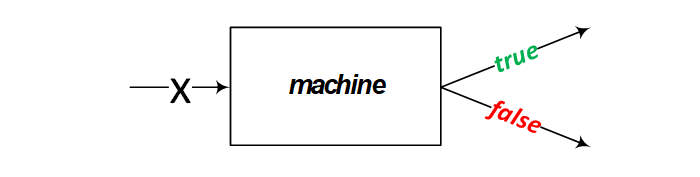
\includegraphics[scale=1]{41.png}
\end{center}
That is the first step. Now we will use the computer science tool to actually build this machine together. 
One of the questions that we will be asking is two things, two aspects to this machine. How much time that a clock, how much time does it take to give the solution and how much space does it need?
When I say space, I mean, for in the case of this mechanical calculator physical space, how many rooms do we need to hold our machine? Or if we're using a computer, how much memory does it need? We will be returning to this two ideas as we go.

\section{Trial division}

\subsection{Define the problem}

We need to build a machine which can answer a simple yes/no question. Given an input integer n, is n prime?
\begin{center}
	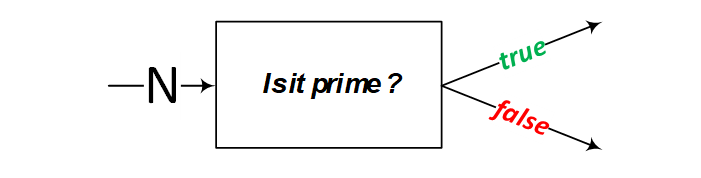
\includegraphics[scale=1]{42.png}
\end{center}
follow a sequence of steps based on some instructions, known as an algorithm. To warm up, let's find out what algorithm is inside your brain. Answer the following question: is 49 prime?\\
No? How did you do that? You likely searched for a divisor of 49 which is greater than 1 and less than 49. If you haven't memorized your multiplication tables then you'd naturally follow this sequence:\\
•	Does 2 divide 49?     NO\\
•	Does 3 divide 49?     NO\\
•	Does 4 divide 49?     NO\\
•	Does 5 divide 49?     NO\\
•	Does 6 divide 49?     NO\\
•	Does 7 divide 49?    YES\\
We found a divisor of 49 (7) which is proof that 49 is composite.

\subsection{Building a wall}
However what if I asked you if 2971215073 is prime?
\begin{center}
	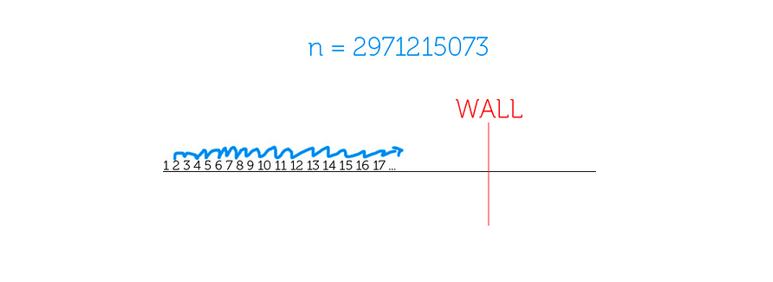
\includegraphics[scale=1]{43.png}
\end{center}
Are you still checking? After the first few thousand tests I still haven't found a divisor. The key question is, when can we stop checking and prove that n is prime? (let's call this our wall) As a starting point, we know our wall must be n-1 (since n divides n). If we check up to 2971215072 either we find a divisor (which proves n is composite) OR we don't (which proves n is prime).
\subsection{Building a better wall}
This would work, but can we move our wall to save time? Remember, that we are actually searching for the first (or smallest) divisor. Sometimes the smallest divisor could be 2, though it could also be much larger. This brings us to the key question: how large could the smallest divisor be?\\
Remember that any composite integer n is build out of two or more primes n= P * P * …
 *P is largest when n has exactly two divisors which are equal to each other.\\ This is known as a square number such as 9 (9 = 3*3) or 49 (49 = 7*7). To capture this worst case scenario we simply build our wall at the square root of n!
\begin{center}
	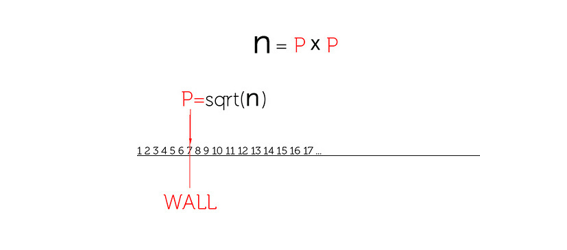
\includegraphics[scale=1]{44.png}
\end{center}
Convince yourself of this: if we don't find a divisor of n after checking up to square root of n, then n must be prime. Try to prove this to yourself (a proof is at the bottom of this article)
\subsection{Trial division algorithm}
That's it, we are ready to move on. First let's summarize our trial division algorithm in plain english:\\
•	Accept some input integer n\\
•	For each integer x from \{2 ... $\sqrt(n)$\} check if x divides n\\
•	If you found a divisor then n is composite OR ELSE n is prime\\
\begin{center}
	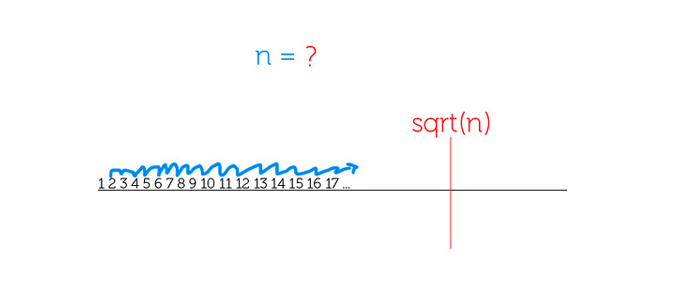
\includegraphics[scale=1]{45.png}
\end{center}

\section{What is computer memory?}
When we perform calculations with a pen and paper, we often need to save intermediate results. And we may do this with, say, scrap paper, and in this case, the paper is acting as a form of external memory. And memory no matter the form, takes up physical space.\\
Computers contain memory, we can think of it as the scrap paper for the computer. And, say, when you construct an array to store values in your program, you require memory. And, at the lowest level, computers read and store all instructions as a string of numbers. But, how do you store numbers in a machine? 
\begin{center}
	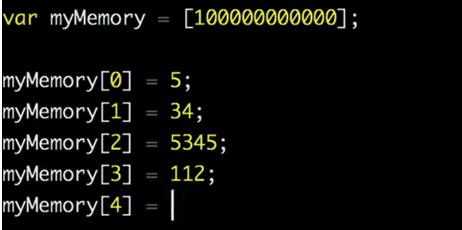
\includegraphics[scale=1]{46.png}
\end{center}
This was a very difficult problem originally, especially when you need computers to hold their memory after the access to power is lost. This is known as nonvolatile memory. The easiest difference for a machine to detect is simply a presence versus an absence of something. \\
So, computers really have 2 fingers, base 2, same as a light switch being "on" for 1, and "off" for 0. This is the smallest amount of information, a single difference, which we call a bit. But bits are powerful for storage because the amount of unique states grows exponentially as we add bits together. Remember, one light switch is one bit and it can store 2 states, but 2 light switches can store 4 unique states. And 8 light switches or 8 bits can store 256 unique states. And space is measured in bits, but the physical size of a bit depends on your method of storage. So how do computer store zero's and one's internally?\\
Modern data processing systems like these use thousands of magnetic cores. What are magnetic cores? They are tiny rings of nickel alloy or other magnetic materials. They have replaced vacuum tubes for many important functions in data processing systems. 
\begin{center}
	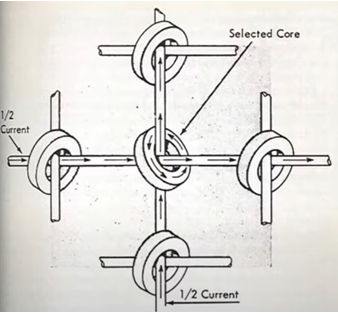
\includegraphics[scale=1]{47.png}
\end{center}
And it allowed computers to store bits as clockwise versus counter-clockwise magnetization direction. Because the each core could be magnetized in 2 different ways, depending which direction the current was applied. \\
Because a bit can be represented by any bi-stable device and a magnetic core is a bi-stable device. Later on, this was done using thin film magnetic disk where we can think of as each bit as a tiny magnetic cell, which can be charged to store either a 1 or a 0. So, long story short, the size of a bit has been rapidly shrinking since the days of punch cards. A hard drive in a modern computer can be thought of as billions of tiny magnetic cells. \\
Now, you may wonder, well how small can these little magnetic cells be? And current research at IBM is pushing this to the atomic level where they have shown 12 iron atoms can work together as a stable magnetic unit, where they are able to store a 1 or a 0, depending how they are oriented. And this is approaching a theoretical limit where we would hold a single bit on a single atom!\\
And interestingly, IBM estimates that we can put around one quadrillion bits of information in a handheld device, the size of an Ipod, with atomic storage. And, let's call this a super drive, it doesn't even exists yet, as a hypothetical example. A small handheld super drive using atomic storage would hold one thousand terabits, which is one thousand trillion switches or more commonly known as 125 terabytes in the palm of your hand, or to use an example everyone can understand, 125 terabytes is the same as having a 1250 kilometer long book shelf in the palm of your hand. \\
And this is what the future of memory looks like, or we ever be able to store a bit on something smaller than an atom?

\section{Sieve of Eratosthenes}
We are now going to introduce an ancient method for generating a list of primes up to some limit N, called the Sieve of Erathosthenes. Now Erathosthenes was born in 276 BC. So this method was over 2200 years old. But it's very simple and elegant and you can teach it to any child. Now let's say for example we want to calculate all the primes up to 100, this would work in the same way if we wanted to calculate up to 10,000 or a billion. Proceeds as follows, assume all numbers are unmarked, grey is unmarked. We start at the beginning and if we find a number that is unmarked we know it's prime. 
\begin{center}
	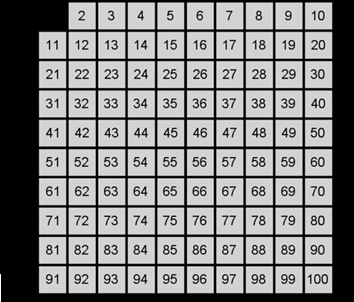
\includegraphics[scale=1]{48.png}
\end{center}
So we hit two and we say two is primed because it's unmarked. And then the second phase is now we can eliminate all multiples of two because we know their composite.
\begin{center}
	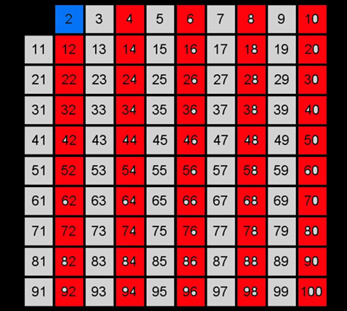
\includegraphics[scale=1]{49.png}
\end{center}
 So bam, we jump along and we eliminate all multiples of two, red means composite. And now we repeat. We step along from two to three. Three is unmarked so we mark three as prime. And now we can eliminate all multiples of three. And a really simple optimization is, notice six is already crossed off, we actually cross off the multiples starting at the square of that number.
\begin{center}
	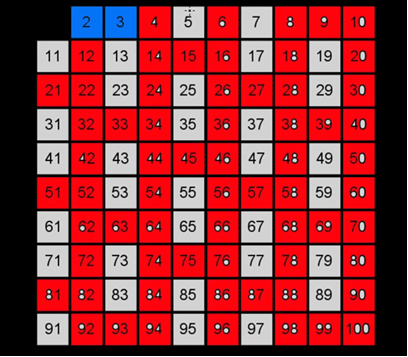
\includegraphics[scale=1]{50.png}
\end{center}
 So three times three is nine. We start at nine and mark all multiples of three as composite. And then again we go back, we jump along to four. Well four is marked, we know it's composite. We jump along to five, we find an unmarked number, five is prime.
\begin{center}
	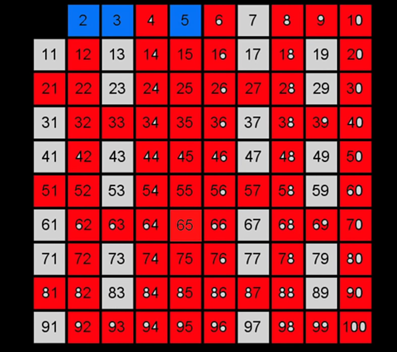
\includegraphics[scale=1]{51.png}
\end{center}
 Now five times five is 25, we go to 25. We mark off 25, 30, 35, 40, 45, and so on. Those are composites. We proceed forward until we hit seven, we know seven is prime because it's unmarked. Seven times seven is 49, we mark 49 and all multiples of seven above it as composite. Now we move along until we hit 11, 11 is prime. Notice now, 11 times 11 is greater than 100, so we can actually stop at this point. We could have stopped at 10 even, because now all remaining unmarked numbers, if you'll notice, are prime.
\begin{center}
	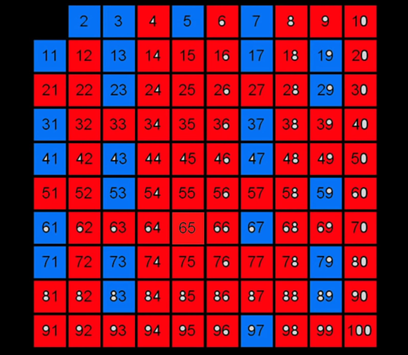
\includegraphics[scale=1]{52.png}
\end{center}
 And in one swoop we can mark them all as prime. And that's the whole algorithm, it's so simple. And just to generalize how we do this, so we could write up a program to perform this sieve, is if we want to find all the primes up to some number N, we first create a main loop.\\
\begin{algorithm}[H]
	\vspace{3mm}
	For all numbers a:from 2 to $\sqrt{n}$\\
		\qquad IF a is unmarked THEN\\
		\qquad \qquad	a is prime\\
		\qquad \qquad	for all multiples of (a<n)\\
			\qquad \qquad \qquad	mark multiples as composite
	
	All unmarked numbers are prime
	\caption{find primes up to N}
\end{algorithm}
So we have four all numbers A, from two to the square root of N. So notice here, we stopped when we hit 10, I showed it as 11, we actually stop because we have found all primes.\\
So from two to the square root of N, we proceed as follows: If A is unmarked, then we know A is prime and when we find a prime number we mark all multiples of A off it's composite and that's it.\\
So, you find a number prime, mark of the multiples, go back to the beginning, increment A by one. So we're at two then we go to three then we go to four, five and so on, and when we're done, we have all primes.\\
Notice here that this is also a loop. So we have a main loop for when we find a prime. This marking off of multiples is also a loop. So it's important to notice here that we have a nested loop, we have a loop inside a loop. 
\newpage
\section{Primality test with sieve}
Now, to recap We are checking if sum number N is prime by doing a trial division. 
\begin{center}
	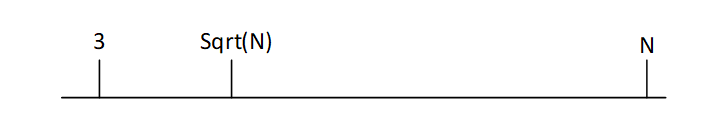
\includegraphics[scale=1]{53.png}
\end{center}
Here is the square root of N and here is three. Starting at three, we are hopping along by two up until the square root of N. At each point in the way, checking if that point divides N. Now so far, people have been trying to reduce the number of steps we take by perhaps starting later and taking larger steps. I just want to pause here and let's think about what is the ideal case for a trial division algorithm? What is the best we could possibly do if we got very creative in our stepping? \\
Remember, any number N has some tri-factorization. Let's say the square root of N is here. We actually only need to step on prime numbers. That would be the best we could do. We know if we step only on primes, we will eventually find a factor. 
\begin{center}
	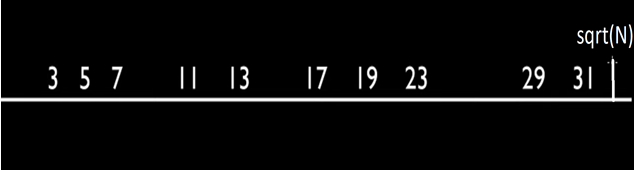
\includegraphics[scale=1]{54.png}
\end{center}
Tri-factor if it's a composite. The question now is how efficient is this method?\\
It seems like we have a perfect solution now. If we wrote a new algorithm which first called the sieve. Let's say the new algorithm is calculating if N is prime. If you call the sieve and generate a nice long list of primes for us. Then, we have our trial division, which would use this list of primes. It would hop along and hit only primes up until the square root of N, wherever that is. What's wrong with this? \\
 Now you may be wondering "Well, what if we calculated the primes in advance?" The first step would be to build an array of primes and store it on a hard drive. Then, our algorithm would just do trial division and it would know how to hop on primes only because it would be reading from this proposed prime list. Perhaps our prime list stores all primes up to 20 digits or even 100 digits. Why can't we do this? \\
The problem is limitations in memory. When we innumerate lists of numbers, which we will explore next. Just for example, let's say we were doing this by hand. We calculate five was prime, we write five on a piece of paper, and we store it in a filing cabinet. Then we get seven, we store that in the filing cabinet., or 11, , into the filing cabinet. Then we have a filing cabinet full of prime numbers. This is our- think of it as a prime array. How big would this filing cabinet be if, say, we wanted all primes up to 20 digits or all primes up to 100 digits long? Could we even store this array on a hard drive? \\
To understand why this actually is not possible we have to dive a little deeper into how large does this actually grow, this prime array, and what is the size limitation of modern-day and even future computer hardware?

\section{The prime number theorem}
Imagine we listed all integers in a growing spiral, and colored the prime numbers blue, and left the composite numbers black. 
\begin{center}
	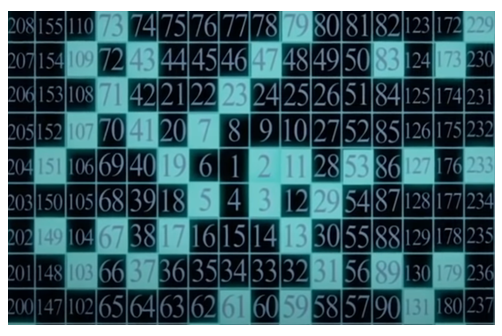
\includegraphics[scale=1]{55.png}
\end{center}
One interesting question we may ask is, "How many primes are there compared to composites?" First, let's zoom out to see the big picture.
\begin{center}
	\includegraphics[scale=1]{56.png}
\end{center}
Notice the prime color is dense in the center, and slowly drops off in the distance but never seems to end. One way I like to think about this is as follows:\\
Imagine there is a tree at the center which is infinitely high. The leaves which drop from this tree represent prime numbers, which are scattered unpredictably below, dense near the base of the tree, and as we walk away from this tree, we find fewer leaves, though we always find them. This is exactly what happens when we look at larger and larger integers. We always find more primes, though the number of primes we find gradually drops, the further we look.\\
So let's return to our question. How many primes are there less than some integer x?\\
If we make a table, we see the number of primes is always increasing. Though as we search further, we find fewer and fewer.
\begin{center}
	\includegraphics[scale=1]{57.png}
\end{center}
 Let's graph the number of primes found on the vertical axis, and the search size x on the horizontal. As we zoom out to include billions of numbers, notice the curve never flat lines. It's always rising, albeit gradually.
\begin{center}
	\includegraphics[scale=1]{58.png}
\end{center}
First, let's think about the density of primes less than some integer x.\\
We can find the density by dividing the number of primes found by the search size. For the first 100 integers, we find 25 primes, therefore 25\% are prime. Of the first 10000 integers, we find 1229 primes, 12.29\% are prime. Of the first 1 million integers, 7.84\% are prime. And the first 100 million integers contain 5.76\% prime. As we search further, this density continues to drop, though the speed at which it drops slows down.\\
Here is a graph of the search size on the horizontal axis and the prime density on the vertical.
\begin{center}
	\includegraphics[scale=1]{59.png}
\end{center}
 Notice that as we zoom out, the primes are a vanishing proportion of all integers. Amazingly, we find this formula in nature. We see it in galaxies, storms, flowers, and even inside our bodies as the design of least resistance, known as the logarithmic spiral. Notice that as the spiral rotates, it gets further and further away from the center. Incredibly, the rotation rate of a logarithmic spiral is related to the density of primes as follows: We have the number of rotations, call this phi. and the distance from the center, call this r.
\begin{center}
	\includegraphics[scale=1]{60.png}
\end{center}
\begin{center}
	\includegraphics[scale=1]{61.png}
\end{center}
 If we graph phi against r, and zoom out, we see they are related according to the natural logarithm. This means the natural logarithm of the distance is related to the number of rotations.
\begin{center}
	\includegraphics[scale=1]{62.png}
\end{center}
The graph of the natural logarithm is commonly written using the variable names y and x as y equals the natural logarithm of x. Notice the graph tapers off in the same way the density of primes gradually decreases. The final step is to invert this by changing the y axis to 1 divided by the natural logarithm of x. And when we zoom out, we find the exact same curve generated when we plot the density of primes. 
\begin{center}
	\includegraphics[scale=1]{63.png}
\end{center}
Let's confirm this by overlapping the two plots. In green, is a graph of the line y equals 1 over the natural logarithm of x. And in red is the plot of prime number density up to x.
\begin{center}
	\includegraphics[scale=1]{64.png}
\end{center}
As we zoom out, they approach each other. The further we zoom out, the more accurate the green estimate becomes. This is known as the asymptotic law of distribution of prime numbers. We now have a formula to accurately tell us the density of primes without counting. The density of primes up to some integer x is approximately 1 divided by the natural logarithm of x or lawn x. So let's say you need to know the density of primes between 1 and 100 trillion. Simple. 1 divided by lawn of 100 trillion equals 3.1\%. Compare this to the actual result from counting all primes which is 3.2\%. This is off by 0.1\%. And as we check larger and larger numbers, the difference approaches zero.\\
Realize now that we can use this formula for prime density to estimate the number of primes up to x. The number of primes is the area under the density curve for which we can simplify by assuming density is constant. So number of primes equals size × density or $\frac{x}{\ln(x)}$    . This is the prime number theorem\\. 
Here is a graph of y equals x divided by lawn x in blue, and in yellow, is a plot of an actual count of primes.
\begin{center}
	\includegraphics[scale=1]{65.png}
\end{center}
 Notice as we zoom out, these lines eventually overlap as we look to infinity. And that is it. We have a formula which tells us approximately how many primes there are up to any value, no counting needed. For example, let's say we need to know the number of primes less than 100 trillion. 100 trillion divided by the natural log of 100 trillion equals 3.1 trillion. Compare this to the actual count, which is 3.2 trillion. This is over 99.99\% accurate even at this relatively small scale.
So to recap: Given a search size up to some integer x, the prime density is about 1 divided by lawn x And the number of primes is about x divided by lawn x. This is the prime number theorem.
\begin{center}
	\includegraphics[scale=1]{66.png}
\end{center}

\section{Time space tradeoff}

We want to introduce the idea of time space trade off, or space time trade off, a commonly used term in computer science. I was looking at a program done by IV46 and they had a million prime array so that there algorithm could step along on primes only, as far as possible, when doing a trial division primality test. It begs the question, why just not store all the primes we need, up to some limit in an array instead of calculating them on the fly?\\
We mentioned in a previous part that this would be optimal for a trial division algorithm. Although you may see his algorithm does not use many steps, it began to run very slowly and eventually crashed before hitting the step limit. So it wasn't able to quickly solve the problem for the sizes I defined earlier. And in this case, they were trading off time in the form of repeated divisibility tests at the expense of space, which is memory to hold the array. Now, why didn't this work? Well, let's do a rough calculation using what we've learned to find out if this method is possible using our memory limit. Remember, we must be able to deal with numbers up to just over 9 quadrillion. Our trial division algorithms only need to check for factors up to the square root of a number, and if it hits that point with no factors found, it can say 100\% whether or not the number is prime. Now, how many primes up to the square root of this limit, where the square root of 9 quadrillion is 94.9 million? How many primes under 95 million?\\
Well, luckily we have learned a mathematical solution to approximate this answer using the prime number theorem. So how many primes are there under x?\\
Well, it's x divided by the natural logarithm of x. And if x is just over 94.9 million, we find the number of primes is approximately 5.1 million. Now because we are storing these primes, we need to know the size of the largest prime, or in this case, the 5.1 millionth prime approximately, which we know will be some number less than 94.9 million. Now, I double checked the table, and the actual value of this prime, the largest prime we would need to store under the square root of our limit, is 89,078,611. Now how much memory does this single large prime number require? Well, to find out, let's convert the number into binary notation, which is how the computer will store the number using tiny switches in memory. We learned about this in the computer memory video. In bits, the largest prime looks like this, which is 24 bits or 3 bytes needed to store this single number. So let's say we want to store each number in memory and since we know the largest number requires 24 bits, we can just imagine a long list of 24 bit blocks storing each prime number. So how many bits are needed for this entire list? Well the memory needed is the number of values, or the number of primes, times the space per value. So we have around 5.1 million values times 24 bits per value, which is just over 124 million bits, or if we convert it into bytes, it's about 14.7 million bytes.
\begin{center}
	\includegraphics[scale=1]{67.png}
\end{center}
Call this almost 15 megabytes. So it is not possible to store even a list of these numbers in memory using our limit. This is just a toy example. It's actually an underestimation of what you'd really need. For example, an array needs space for a pointer to each item, and each pointer on a 32 bit machine is 4 bytes. So the actual amount of memory needed is much more than 15 megabytes. That being said, we know that storing all primes up to the square root of our relatively small limit is not even possible with our memory limit. We can't do it this way. \\
Okay, well, what about when prices drop by a factor of a thousand, or ten thousand. Modern day cryptographic systems use 512 bit, or even larger numbers, making search and enumeration impossible. Now for example, if someone asks you to make a list of all prime numbers up to primes which are 200 digits in length, you shouldn't even consider it because the hard drive needed to store all these primes would be heavier than the mass of the observable universe. I'll leave the calculations for you to try next time you're at a restaurant with crayons and paper all over the table. But remember, there are around 10 to the 80 atoms in the observable universe. That's an 80 digit number.\\ 
Realize now, there is a fundamental limit for how much space or memory we have access to. Nevermind how much time it would take, but there is always this push and pull between using space or time to solve our problems. So to solve this problem of testing for primality quickly using a small amount of space, and a small amount of time, we are going to have to approach it in an entirely new way.\\
\section{Summary (what's next?)}
Congratulations. We've reached a branching point in our lesson. Now a few different ideas have been introduced, so it's important to orient ourselves here before moving forward in various directions. Now, what motivated this lesson? \\
Well, we learned about RSA encryption, and RSA depended on two things. One, that prime factorization is difficult. So if I multiply two big primes together, P1 and P2 and I give you N, I can trust or feel secure in knowing that you'll take a long time to find those primes, and maybe more than your lifetime. Also two, RSA requires that those large primes I generated was easy, meaning I could just quickly generate a large prime. So let's return to the first problem. Difficulty of prime factorization.\\
Well what is it about prime factorization or just prime numbers themselves which make problems hard? And to find out we begin with a core problem. Given X, is X prime or composite, which is a primality test? \\
Now we ended up building some solutions to this problem. And in doing so, we realize that this problem was computationally expensive. That is, there is no instant solution to this problem. As our input number grew, the amount of time or the amount of steps involved for an algorithm to find the solution also grew. And, how much it grew, we actually understand better now because we can predict this search space using the prime number theorem. \\
Though, the real issue can be thought of as a graph, where on the vertical axis we have the number of steps our algorithm takes, so you can just think of it as time. And on the X-axis is the input size and as input size increased, so did time. And the problem we had is that shape of this curve is unacceptable.
\begin{center}
	\includegraphics[scale=1]{68.png}
\end{center}
Because in our case, once N hit even 20 digits, we can no longer solve the problem in the worst case. And if we threw in input hundreds of digits long at our algorithm we can all agree it would not work. In our case it would crash. So it's practically impossible to check if large input is prime using our current strategies. \\
Now let's return to the first point, factorization. Realize based on our current understanding in this lesson, factorization has to be harder than a primality test. \\
That is there are more steps involved in finding the prime factorization of some number, versus just telling me if a number is prime. Since, remember, factorization requires us to find all the prime factors for some input N, whereas a primality test only requires we find one divisor And a nice reminder of this is that some users have actually turned these primality tests into prime factorization algorithms, simply by repeating after it finds its first divisor. So the primality test is just kind of a sub-routine inside the main factorization algorithm. So if we return to that graph, a factorization algorithm would be something like this.\\
As input grows, our factorization algorithm would be above this primality test line. And realize that in any situation we always have a computational limit, that is the number of primitive steps we can calculate which is based on our computing power in any given situation and the amount of time we have. And you could think of this as a horizontal line, or a threshold on this graph.
\begin{center}
	\includegraphics[scale=1]{69.png}
\end{center}
 Anything above this line is out of reach, not feasible to solve. \\
And in this lesson we were limited by the rover's on-board computer which was fairly slow, which is why we couldn't run primality tests on numbers with even 20 digits. However, even if we had, say, 1,000 computers running for a year, this would simply just push this horizontal line up to some other threshold. 
\begin{center}
	\includegraphics[scale=1]{70.png}
\end{center}
And this would allow us to run tests on larger numbers, but as you can see, we would always hit some limit where the input is large enough that we can no longer solve the problems again. \\
Now, this leads to many interesting question paths. However, I'll identify the two I'm going to explore next. First of all, so far I have not been very precise about these growth curves. Though, it would be helpful if, imagine for any algorithm you give me, no matter what it's trying to solve, and no matter what machine it's even running on, we could draw some corresponding growth curve on this graph, simply by looking at the description of the algorithm. If we could do this, we could identify categories of certain growth shapes, which tell us how difficult a problem would be to solve. And in this way, we could understand an algorithm before we even run it, very important to think about. And you could hand me your algorithm written on a piece of paper and I could look at it and I'll say, "I know "this algorithm is not solvable with the input size needed." And this leads us to a lesson on time complexity, an incredibly important conceptual tool we will need. And if you've ever heard this runs in polynomial time or exponential time, these are terms which come out of time complexity.\\
Next, many of you have been wondering, "well, how "are we generating these random primes in practice," the second point I made about RSA. Well let's just walk through it quickly. To generate a large random prime number hundreds of digits long, we need to follow these instructions.\\
Generate a random number, test if it's prime, if it's prime, we're done. If not, try again until we hit a prime. \\
Now in this three-step procedure, what's most important is the second step, test if it's prime. If we can't do that step, this won't work. So how is this working today?\\
Well, it's based on a subtle alteration to our problem definition, and more importantly, the use of randomness. And this leads us to another lesson on random algorithms. 

\chapter{Randomized algorithms}
\newpage
Now my question is would access to randomness help us speed up a decision algorithm such as this primality test? 
This is a deep question, so let's step back and look at the big picture. 
\begin{center}
	\includegraphics[scale=1]{71.png}
\end{center}
Given some collection of integers from one to some limit N say, let's think of it as our universe of integers. We can always divide a collection into two sets. A decision problem can actually be thought of as a partition into two sets. For example, provided some N is N less than 100, it will output yes for all integers less than 100. Here is one collection, and no for all others, which is another collection. Okay, so let's now focus on recognizing primes with the decision. Ideally, what we would like is some simply computed criteria that all primes satisfy and no composites satisfy.
\begin{center}
	\includegraphics[scale=1]{72.png}
\end{center}
 Now if we knew some simple pattern which describes the location of all primes, and only primes, then given some number N we could simply check if N follows that pattern. The problem is that so far no exhaustive and simply computed pattern has been found for all primes and no composites, or all composites and no primes. But we do know fast tests for most composite numbers. For example, a simply computed criteria would be a test for evenness, and all even numbers are divisible by two.
 \begin{center}
 	\includegraphics[scale=1]{73.png}
 \end{center}
It's fast because we can tell if something's even by just looking at the last digit, and even as N grows, the problem doesn't get any harder, we just look at that last digit also known as the low order bit. Now realize that we can use this evenness test as a low quality composite test. In that we could have some algorithm accept our integer N, and all our algorithm does is check if it's even. If it is even, and greater than two, then we know with 100 percent certainty it is composite because we have proof. Think of two as our composite witness. However if not, then we aren't exactly sure. If it's odd it could be prime since all primes are odd, or it could be one of the many composites which are odds, just nine or fifteen. This massive region of odd composites makes for an unacceptable test. Now to be clear, let's draw this. Provided some N, N can be either prime or composite. If N is prime, our algorithm will say prime 100 percent of the time since no primes are even that are greater than two. It will never say composite when a prime is provided. However, if N is composite, our algorithm will say composite about fifty percent of the time, and prime fifty percent of the time. This means that if our algorithm outputs composite, it means it found proof of composite witness. However, for our algorithm outputs prime, we know there is an unacceptably large chance of error. \\
Until now, our strategy has dealt with this large, unacceptably large error, by iteration and let's draw the flow of our machine. Given some N, our machine does a series of divisibility tests starting at A is two. It asks does A divide N. If it doesn't divide N, then we can eliminate all of this region. Then it asks the next question, does N divide three? If not, then we eliminate that whole section. Does N divide five, seven, and so on. Notice these are disjoint sets which gradually fill up all possible composites. Now if we ever answer yes along the way, then we have proof that N is composite. A, whatever it is at that point, is our witness. We halt N output composite from our algorithm. Otherwise, we continue trying until we exhaust all possible composites. Until we hit the square root of N since we know, remember ever composite number N must have a factor less than or equal to the square root of N. This really leads to the final question in our algorithm. If no witnesses are found, and A is greater than the square root of N, then we suddenly have proof and we halt an output prime. Realize we have two exit paths through our algorithm. Both paths represent proof of certainty that N is either prime or composite. When N is prime, we try all possible divisors and we basically rule them all out, and that is our proof that N is prime. \\
The problem with this strategy is that our test value A at minimum requires us to cycle through every prime starting from two to the square root of N. As N grows, the number of primes grow with it. It results in too many iterations in the worst case such as when we provide a prime to our algorithm. Looking at the big picture now, realize it's providing proof when N is prime. Which we now know we don't exactly need. No one said we needed to prove it. We just needed to be 99.9999 fifteen nine's percent certain. Hmm, so we actually need to think about the composite test that's being used in our algorithm. Remember, our fastest trial division primality tests thus far have tried to use prime pattern such as 6K, or all primes are of the form 6K plus or minus one, to help walk along the primes only and eliminate many of the composites to save time. Remember, a test like this can be turned into a composite test. That is, given some integer N is of the form 6K plus or minus one, then we can say it's probably prime, but there are many composites still which follow this pattern. It doesn't include primes only, just all primes and some composites, and we can think of these extra composites as a leak and this leak is our source of error.\\
Now if we invert it and ask is N not of the form 6K plus or minus one, then we can say with 100 percent certainty it is composite, so the leak is our source of error on the prime side, but in this case it's unacceptable it's not a non-negligible error. There's a much larger probabilty. We need to define a new composite testing procedure which is able to shrink this space and make the chance of error negligible. Which means we'll need to review how we can actually shrink errors with iterations. 

\section{Conditional probability explained visually}
Consider the following story. 
Bob is in a room and he has two coins. One fair coin and one double sided coin. He picks one at random, flips it, and shouts the result.  Now what is the probability that he flipped the fair coin? To answer this question, we need only rewind and grow a tree. The first event, he picks one of two coins, so our tree grows two branches, leading to equally likely outcomes, fair or unfair. The next event, he flips the coin. We grow again, if he had the fair coin, we know this flip can result in two equally likely outcomes, heads and tails, while the unfair coin results in two outcomes, both heads.
 \begin{center}
	\includegraphics[scale=1]{74.png}
\end{center}
Our tree is finished, and we see it has four leaves, representing four equally likely outcomes. The final step, new evidence, he says. \\
Whenever we gain evidence, we must trim our tree. We cut any branch leading to tails because we know tails did not occur, and that is it, so the probability that he chose the fair coin is the one fair outcome leading to heads divided by the three possible outcomes leading to heads, or one third.
 \begin{center}
	\includegraphics[scale=1]{75.png}
\end{center}
 What happens if he flips again and reports?\\
after each event, our tree grows. The fair coin leaves result in two equally likely outcomes, heads and tails, the unfair coin leaves result in two equally likely outcomes, heads and heads. 
 \begin{center}
	\includegraphics[scale=1]{76.png}
\end{center}
After we hear the second. We cut any branches leading to tails.Therefore the probability the coin is fair after two heads in a row, is the one fair outcome leading to heads divided by all possible outcome leading to heads, or one fifth. 
 \begin{center}
	\includegraphics[scale=1]{77.png}
\end{center}
Notice our confidence in the fair coin is dropping as more heads occur, though realize that we'll never reach zero. No matter how many flips occur, we can never be 100\% certain the coin is unfair. \\
In fact, all conditional probability questions can be solved by growing trees. Let's do one more to be sure.\\
Bob has three coins, two are fair, one is biased, which is weighted to land heads two thirds of the time and tails one third. He chooses a coin at random and flips it. – Bob : Heads. Now what is the probability he chose the biased coin? Let's rewind and build a tree. The first event, choosing the coin, can lead to three equally likely outcomes, fair coin, fair coin, and unfair coin. The next event, the coin is flipped. Each fair coin leads to two equally likely leaves, heads and tails. The biased coin leads to three equally likely leaves, two representing heads, and one representing tails. 
 \begin{center}
	\includegraphics[scale=1]{78.png}
\end{center}
Now the trick is to always make sure our tree is balanced, meaning an equal amount of leaves growing out of each branch. To do this, we simply scale up the number of branches to the least common multiple. For two and three, this is six. And finally, we label our leaves. The fair coin now splits into six equally likely leaves, three heads and three tails. For the biased coin, we now have two tail leaves and four head leaves, and that is it.
 \begin{center}
	\includegraphics[scale=1]{79.png}
\end{center}
 When Bob shouts the result. - Bob : Heads. -This new evidence allows us to trim all branches leading to tails since tails did not occur, so the probability that he chose the biased coin given heads occurred, well four leaves can come from the biased coin divided by all possible leaves. Four divided by 10, or 40\%. 
 \begin{center}
	\includegraphics[scale=1]{80.png}
\end{center}

When it doubt, it's always possible to answer conditional probability questions by Bayes Theorem, it tells us the probability of event A given some new evidence B, though if you forgot it, no worries.
\dfn{Conditional Probability}{
$$P(A|B)=\dfrac{P(B|A)*P(A)}{P(B)}$$
}

\section{Random primality test}
First, let's build up the conceptual mechanics for these new types of random algorithms which accept some input N and if N is prime, our algorithm will output prime with 100\% certainty.
 \begin{center}
	\includegraphics[scale=1]{81.png}
\end{center}
 It will never label it as composite. However, if N is composite, there will be some tiny chance of error E that it will label it prime. Otherwise, there is a one minus this tiny error probability that it will correctly identify it as composite.\\
We will start simple. Out of some universe of integers up to some limit, we grab a number and call this integer N. We input N into our machine. Previously, in our trial division methods, we basically iterated through all values from one to the square root of N and tested if that number divides N. 
 \begin{center}
	\includegraphics[scale=1]{82.png}
\end{center}
Ideally, we only wanted to check primes to save time. If yes, A divides N, we know that N is a composite number because we found a composite witness. If not, we aren't sure. So, we go back and we increment A and we test again. Once we exhaust all possible tests, we can then say yes, N is prime, if we found no divisors.\\
Now, let's be lazy. What if we just pick a few random integers and do a few divisibility tests which you can think of as random questions. We know that some number N, if it is composite, it must have some divisors scattered around. At minimum, it has a single divisor. Some composite numbers have many divisors. Anyway, we pick a random integer A between one and the square root of N. That's it. Then we just check if A divides N. As before, if A divides N we know for sure that N is composite, we found a witness. If not, we haven't learned too much except that it could be prime. To be safe, we could generate a few more random As and keep testing. Perhaps after 100 or 1,000 iterations, we could stop and say "It's probably prime" with some certainty. Say, for example, 99.9 percent. \\
We need to use another test. We need an equation which is fast to calculate, that can be used to prove whether a number is composite. It must accept not only the input integer N, but also a random integer A and do a random test in the same sort of way.

\section{Fermat's little theorem}
Bob discovered something very interesting while making multicolored earrings out of beads for his store. Now, his customers like variety, so he decides to make every possible style for each size.
 \begin{center}
	\includegraphics[scale=1]{83.png}
\end{center}
 Starting with size three, he begins by figuring out all possible styles. Each earring begins as a string of beads, and then the ends are attached to form a ring. So first, how many possible strings are there? With two colors and three beads, there are three choices, each from two colors. So two times two times two equals eight possible unique strings.And then he subtracts the strings which have only one color, or monocolored strings,since he's only building multicolored earrings.
 \begin{center}
	\includegraphics[scale=1]{84.png}
\end{center}
 
Then he glues them all together to form rings. He was assuming he would end up with six different earrings, but something happened. He could no longer tell the difference between most of them. It turns out he only has two styles, because each style is now part of a group with two identical partners. Notice you can always match them up based on rotations. So the size of these groups must be based on how many rotations it takes to return to the original. Or how many rotations to complete a cycle. So this means that the original set of all multicolored strings divides evenly into groups of size three.

 \begin{center}
	\includegraphics[scale=1]{85.png}
\end{center}
Now, would this be true for other sizes? That would be convenient, since he always wants the same amount of each style. So he tries this with four beads. First he builds all possible strings. With four beads he can choose from two colors for each bead, so two times two times two times two equals sixteen. Then he removes the two monocolored necklaces and attaches all of the others to form rings.\\
Now, will they form equal sized groups? Apparently not. What happened? Notice how the initial set of strings divides into styles. If strings are of the same style, it means you can form one into the other simply by grabbing beads from one end and sticking them onto the other end. And there is one style which only has two members, and this is because it's built out of a repeating unit of length two. So only two rotations are required to complete a cycle. Therefore this group only contains two. He cannot split them into an equal number of styles.
 \begin{center}
	\includegraphics[scale=1]{86.png}
\end{center}
 What about size five? Will they break into equal number of each style? Wait, suddenly he realizes he doesn't even need to build them in order to find out. It must work, since five cannot be made up of a repeating pattern, because five cannot be broken up into equal parts. It's a prime number. So no matter what kind of multicolored string you start with, it will always take five rotations, or bead swaps, to return to itself. The cycle length of every string must be five. Well let's check. First we'll build all possible strings and remove the two monocolored strings.
 \begin{center}
	\includegraphics[scale=1]{87.png}
\end{center}
 Then we separate the strings into groups which belong to the same style, and build a single earring for each style. Notice that each earring rotates exactly five times to complete a cycle. Therefore, if we glued all the strings into rings, they must split into equal sized groups of five. But then he goes one step further. Currently he is only using two colors, but he realizes this must hold with any number of colors. 
 \begin{center}
	\includegraphics[scale=1]{88.png}
\end{center}
Because any multicolored earring with a prime number of beads, P, must have a cycle length of P, since primes cannot be broken into equal sized units. But if a composite number of beads are used, such as six, we will always have certain strings with shorter cycle lengths, since it's actually built out of a repeating unit, and therefore will form smaller groups. And amazingly he just stumbled onto Fermat's Little Theorem. Given A colors and strings of length P, which are prime,
$$a=\text{number of colors}$$
$$p=\text{length}$$
 the number of possible strings is A times A times A, P times, or A to the power of P. And when he removed the monocolored strings, he subtracts exactly A strings, since there are one for each color. This leaves him with A to the power of P minus A strings.
$$\text{number of strings}=a^p-a$$
And when he glues these strings together, they will fall into groups of size P, since each earring must have a cycle length of P. Therefore, P divides A to the power of P minus A. And that's it. We can express this statement in modular arithmetic too. Think of it, if you divide A to the power of P by P, you will be left with a remainder of A.
$$\dfrac{a^p}{p}=x_{\text{remainder}}a$$
 So we can write this as A to the power of P is congruent to A mod P. 
 $$a^p  \equiv  a \quad \text{mod} \quad p$$
And here we have stumbled onto one of the fundamentals results in number theory merely by playing with beads.
\dfn{Fermat's Little Theorem}{The Fermat's Little Theorem is a fundamental result in number theory, named after the French mathematician Pierre de Fermat. It establishes a relationship between prime numbers and modular arithmetic. The theorem states:\\

If $p$ is a prime number and $a$ is an integer not divisible by $p$, then
\[ a^{p-1} \equiv 1 \pmod{p} \]

Here, $a^{p−1}$ is the remainder when aa raised to the power of p−1 is divided by p, and (modp) represents the modulo operation with respect to p. This theorem has significant applications in various areas of number theory, cryptography, and computer science.\\
Fermat's Little Theorem is a special case of Euler's Totient Theorem, which extends this result to non-prime moduli. It's important to note that Fermat's Little Theorem only applies when a is not divisible by p; if aa is divisible by pp, then the theorem doesn't hold.\\
The theorem is used in many cryptographic algorithms, including RSA encryption, to ensure the security and correctness of the algorithms by exploiting the properties of prime numbers and modular arithmetic.
}

\section{Fermat primality test}
Our goal is to define a series of instructions which can prove whether some input integer is composite or else identify it as prime with some very high degree of accuracy. Which we can define, and it must be efficient to do so. Meaning it should be fast to calculate on any machine and even if the input size grows, which is our input integer N, it should still be fast. And so far we've learned that at the lowest level this requires some known pattern that all primes follow and very few composites follow. However, in the previous part we did a visual demonstration of Fermat's little theorem and it provides us with a very interesting rule. Given some prime number P and some other integer A. Which is just less than P. We know now that P divides A to the power of P minus A. We write this as A to the power of P equals A mod P and that's the way you'll normally see it. Now because A and P share no common factor since P's a prime, we can use a cancellation law, and you'll sometimes see this written as A to the power of P minus one is one mod P, and remember we can only do this because the greatest common divisor of A and P equals one,
$$a^p \equiv a \quad \text{mod} \quad p \quad \Rightarrow \quad a^{p-1} \equiv 1 \quad \text{mod} \quad p$$
\ex{}{
a=10\\
p=181\\
$\Rightarrow \quad 10^{181-1} \quad \text{mod} \quad 181 = 1$
}
\ex{}{
	a=74\\
	p=180\\
	$\Rightarrow \quad 74^{180-1} \quad \text{mod} \quad 180 = 104$
}
 This is now proof that the P we chose cannot be composite, and that's the essence of this test, and before going any deeper, let's just step back and construct the frame work for this test using this pattern I just showed you. \\
So our test starts. We are provided with some integer. Let's call it P, as input. Next we generate a random integer A. Which is less than P, and now we can as, is the greatest common divisor of A and P one? If not, if the greatest common divisor of A and P is greater than one, then they share a common factor and we've proven that P is composite because a factor exists and we can halt and exit and our algorithm will output composite. However, if yes, and we can ask the key question, does A to the power of P minus one mod P equal one? If not, we have a witness that P is composite. We can halt and say we're done, P's composite. Otherwise, if yes, if our equation outputs one, then it should be prime, right?
 \begin{center}
	\includegraphics[scale=1]{89.png}
\end{center}
 I coded up this series of instructions, and on the left hand side we have Fermat's test, and on the right I just have an existing trial division test and that's there because we know that test is always correct and just at first glance it seems like it's working.
 \begin{center}
	\includegraphics[scale=1]{90.png}
\end{center}
 \begin{center}
	\includegraphics[scale=1]{91.png}
\end{center}
 However, I found a problem. I hit the number 511, and now the Fermat's test is saying it's prime, and the trial division test is telling me that it's composite. 511 seems prime from the tests perspective but it's not.
  \begin{center}
 	\includegraphics[scale=1]{92.png}
 \end{center}
 Now let's just return back to our equation and see what happened. Well this is an example of what we call a pseudoprime. It's a composite number but there are certain A's we can choose that will output a one. That's incorrect again. So these A's which result in a composite number outputting a one, we can call fools, because they're fooling us into thinking the number's prime, but notice that if we choose different A's, we seem to find many composite witnesses instead of fools. So we could maybe just step back and let's apply the same logic we used in the divisibility test where we simply repeat the experiment a few times and generate a new random A each time and hopefully we won't pick a fool each time. Now it's been proven that the number of fools must divide the total size of the group we select from. Which means at most, half of the choices or half of the elements in this pool could be fools. So since A is chosen randomly, the chance of finding a composite witness, which is what we want, is at lest one half. After T iterations, the probability that no witness will be found with a composite number is at most one divided by two to the power of T. So after 20 trials the probability of mistakenly outputting a prime is just over one in a million. So that's the case where we just keep getting really unlucky and generating random A's and every time we choose I fool. If you can let that sink in, that's really powerful to understand, and here now we can see our test in action with the increase number of trials. It seems to be working perfectly, and notice that in the worst case, which we know is when we provide our algorithm with a prime, it's gonna do the maximum amount of work. The Fermat test is much more efficient than trial division. Especially because the number of steps doesn't scale with the input and that's a key distinction. We set the number of trials and that's it. We never have to worry about our algorithm running millions and millions of iterations as we did before. So I mean this is quintessentially applied math. We are taking a pattern someone discovered and we're saving an immense amount of computational cycles. However, there is one tiny flaw for error in this system. Can you find it?
 \begin{center}
	\includegraphics[scale=1]{93.png}
\end{center}

\end{document}
